\documentclass[compress]{beamer}
\usetheme{Warsaw}
\useoutertheme{split}

%%%%%%%%%%%%%%%%%%%%%%%%%%%%%%%%%%%%%%%%%%%%%%%%%%%%%%%%%%%%%%%
% Improvement on the default split theme : added line numbers %
%%%%%%%%%%%%%%%%%%%%%%%%%%%%%%%%%%%%%%%%%%%%%%%%%%%%%%%%%%%%%%%

\setbeamercolor{frametitle}{fg=white}
\setbeamercolor{frametitle right}{fg=white}

\defbeamertemplate*{footline}{mysplit theme}
{%
  \leavevmode%
  \hbox{\begin{beamercolorbox}[wd=.5\paperwidth,ht=2.5ex,dp=1.125ex,leftskip=.3cm plus1fill,rightskip=.3cm]{author in head/foot}%
    \usebeamerfont{author in head/foot}\insertshortauthor
  \end{beamercolorbox}%
  \begin{beamercolorbox}[wd=.4\paperwidth,ht=2.5ex,dp=1.125ex,leftskip=.3cm,rightskip=.3cm plus1fil]{title in head/foot}%
    \usebeamerfont{title in head/foot}\insertshorttitle
  \end{beamercolorbox}}%
    \begin{beamercolorbox}[wd=.1\paperwidth,ht=2.5ex,dp=1.125ex,leftskip=.1cm plus1fill,rightskip=.1cm]{date in head/foot}
      \usebeamerfont{date in head/foot} \insertframenumber{} / \inserttotalframenumber
    \end{beamercolorbox}
  \vskip0pt%
}

\defbeamertemplate*{headline}{mysplit theme}
{%
  \leavevmode%
  \begin{beamercolorbox}[wd=.45\paperwidth,ht=2.5ex,dp=1.125ex]{section in head/foot}%
    \insertsectionnavigationhorizontal{.4\paperwidth}{\hskip0pt plus1filll}{}%
  \end{beamercolorbox}%
  \begin{beamercolorbox}[wd=.55\paperwidth,ht=2.5ex,dp=1.125ex]{subsection in head/foot}%
    \insertsubsectionnavigationhorizontal{.6\paperwidth}{}{\hskip0pt plus1filll}%
  \end{beamercolorbox}%
}

%%%%%%%%%%%%
% packages %
%%%%%%%%%%%%

\usepackage{scontents}
\makeatletter
\let\verbatimsc\@undefined
\let\endverbatimsc\@undefined
\makeatother
\usepackage{minted}
\newminted{tex}{linenos}
\newenvironment{verbatimsc}
               {\VerbatimEnvironment
                 \begin{minted}[linenos,escapeinside=||]{cpp}}
               {\end{minted}}
\newcommand\highlightCppCode[2]{
  \renewenvironment{verbatimsc}
                   {\VerbatimEnvironment
                     \begin{minted}[linenos,highlightlines={#1},escapeinside=||]{cpp}}
                   {\end{minted}}
  \typestored{#2}
}
\newminted{cpp}{gobble=4,linenos}
\newminted{shell-session}{gobble=4}
\newminted[makefile]{shell-session}{gobble=4}
\newminted{python}{linenos=true,gobble=4}

\usepackage{pgf}
\usepackage{pgffor}
\usepackage{tikz}
\usetikzlibrary{arrows,automata,snakes,shapes}

\usepackage{tcolorbox}

\usepackage[framemethod=TikZ]{mdframed}
\mdfdefinestyle{simplebox}{roundcorner=4pt,linewidth=0,backgroundcolor=blue!50!black,fontcolor=white}

\usepackage{multicol}
\usepackage{tikz-uml}

\usepackage{booktabs}

%%%%%%%%%%%%%%%%%%%
% useful commands %
%%%%%%%%%%%%%%%%%%%
\newcommand{\cpp}{C$^{++}$}
\newcommand{\deprecated}{\textcolor{red}{\bf Deprecated}}

%%%%%%%%%%%%%%%%%%%%%%%%%%%%%%%
% frametitle with C++ version %
%%%%%%%%%%%%%%%%%%%%%%%%%%%%%%%
% Use as \frametitlecpp[14]{Title}
\newcommand\frametitlecpp[2][98]{
  \frametitle{#2 \hfill \cpp#1}
}
% Deprecated:
% used reverse leet speech for the numbers as a latex command cannot use numbers
% 98 -> gb, 11 -> ii, 14 -> ia, 17 -> it, 20 -> so
\newcommand\frametitlegb[1]{ \frametitlecpp[98]{#1} }
\newcommand\frametitleii[1]{ \frametitlecpp[11]{#1} }
\newcommand\frametitleia[1]{ \frametitlecpp[14]{#1} }
\newcommand\frametitleit[1]{ \frametitlecpp[17]{#1} }
\newcommand\frametitleso[1]{ \frametitlecpp[20]{#1} }

%%%%%%%%%%%%%%%%%%%%%%%%%%%%%%%
% easy class diagrams in tikz %
%%%%%%%%%%%%%%%%%%%%%%%%%%%%%%%

\newcommand\classbox[3][]{
  \def\temp{#3}
  \ifx\temp\empty
    \draw[thick] node (#2) [#1]
         [rectangle,rounded corners,draw] {#2};
  \else
    \draw[thick] node (#2) [#1]
         [rectangle,rounded corners,draw] {
      \begin{tabular}{l}
        \multicolumn{1}{c}{#2} \\
        \hline
        #3
      \end{tabular}
    };
  \fi
}

%%%%%%%%%%%%%%%%%%%%%%%%%%%%%%%%%%%%%%
% easy memory stack diagrams in tikz %
%%%%%%%%%%%%%%%%%%%%%%%%%%%%%%%%%%%%%%

\newcounter{memorystackindex}

\pgfkeys{
  memorystack/.is family,
  memorystack,
  size x/.initial=4cm,
  size y/.initial=.5cm,
  word size/.initial=4,
  nb blocks/.initial=8,
  base address/.initial=12351,
  color/.initial=black,
  addresses/.initial=1
}

\makeatletter

\newcommand\memorystackset[1]{\pgfkeys{memorystack,#1}}
\newcommand\memorystack[1][]{
  \memorystackset{#1,
    size x/.get=\stacksizex,
    size y/.get=\stacksizey,
    word size/.get=\stackwordsize,
    nb blocks/.get=\stacknbblocks,
    base address/.get=\stackbaseaddr,
    color/.get=\stackcolor,
    addresses/.get=\displayaddrs
  }
  \draw[thick,\stackcolor,text=white] node (title)
        at (\stacksizex/2, \stacknbblocks*\stacksizey+.5cm)
        [rectangle,rounded corners,fill=blue!50!black] {Memory layout};
  \setcounter{memorystackindex}{1}
  \draw[thick,\stackcolor] (0,0) rectangle (\stacksizex,\stacknbblocks*\stacksizey);
  \pgfmathsetmacro{\nbbars}{\stacknbblocks-1}
  \pgfmathtruncatemacro\nbbarstrunc{\nbbars}
  \ifnum\nbbarstrunc>0
    \foreach \n in {1,...,\nbbars} {
      \draw[\stackcolor!70] (0,\n*\stacksizey) -- +(\stacksizex,0);
    }
  \fi
  \foreach \n in {1,...,\stacknbblocks} {
    \foreach \p in {1,...,\stackwordsize} {
      \draw node (stack\n-\p)
            at (\stacksizex/\stackwordsize*\p-\stacksizex/\stackwordsize/2,\n*\stacksizey-\stacksizey/2)
            [rectangle,minimum width=\stacksizex,minimum height=\stacksizey] {};
    }
    \ifnum1=\displayaddrs\relax
      \pgfmathparse{\n*\stackwordsize+\stackbaseaddr}
      \pgfmathdectoBase\hexversion{\pgfmathresult}{16}
      \draw node at (\stacksizex,\n*\stacksizey-\stacksizey/2) [right=2pt]
            {0x\hexversion};
    \fi
  }
  \pgfmathsetmacro{\nbseps}{\stackwordsize-1}
  \pgfmathtruncatemacro\nbsepstrunc{\nbseps}
  \ifnum\nbsepstrunc>0
    \foreach \n in {1,...,\nbseps} {
      \draw[\stackcolor!10] (\stacksizex/\stackwordsize*\n,0) -- +(0,\stacknbblocks*\stacksizey);
    }
  \fi
}

\newcommand\memorypushvalue[3]{
  \draw node at (stack#1-#2) {#3};
}

\newcommand\memorypushwidevalue[1]{
  \memorystackset{
    size x/.get=\stacksizex,
    size y/.get=\stacksizey,
  }
  \draw node (content) at (\stacksizex/2,\value{memorystackindex}*\stacksizey-\stacksizey/2) {#1};
  \draw[\stackcolor!80,->] (content) -- (.2cm,\value{memorystackindex}*\stacksizey-\stacksizey/2);
  \draw[\stackcolor!80,->] (content) -- (\stacksizex-.2cm,\value{memorystackindex}*\stacksizey-\stacksizey/2);
  \addtocounter{memorystackindex}{1}
}

\newcommand\memorypushhalfvalue[1]{
  \memorystackset{
    size x/.get=\stacksizex,
    size y/.get=\stacksizey,
  }
  \draw node (content) at (\stacksizex/4,\value{memorystackindex}*\stacksizey-\stacksizey/2) {#1};
  \draw[\stackcolor!80,->] (content) -- (.2cm,\value{memorystackindex}*\stacksizey-\stacksizey/2);
  \draw[\stackcolor!80,->] (content) -- (\stacksizex/2-.2cm,\value{memorystackindex}*\stacksizey-\stacksizey/2);
  \addtocounter{memorystackindex}{1}
}

\newcounter{localcount}
\newcommand\memorypush[1]{
  \memorystackset{
    word size/.get=\stackwordsize,
    nb blocks/.get=\stacknbblocks
  }
  \count@=0
  \setcounter{localcount}{1}
  \@for\v:=#1\do{
    \ifnum\count@<\stackwordsize
      \advance\count@ 1
      \memorypushvalue{\arabic{memorystackindex}}{\arabic{localcount}}{\v}
    \fi
    \addtocounter{localcount}{1}
  }
  \addtocounter{memorystackindex}{1}
}

\newcommand\memorypushpointer[2][]{
  \memorystackset{
    word size/.get=\stackwordsize,
    base address/.get=\stackbaseaddr
  }
  \pgfmathparse{#2*\stackwordsize+\stackbaseaddr}
  \pgfmathdectoBase\hexaddress{\pgfmathresult}{16}
  \memorypushvalue{\arabic{memorystackindex}}{1}{#1 0x\hexaddress}
  \draw[\stackcolor!80,->] (stack\arabic{memorystackindex}-1.west) .. controls +(left:1) and +(left:1) .. (stack#2-1.west);
  \addtocounter{memorystackindex}{1}
}

\newcommand\memorystruct[3]{
  \memorystackset{
    size y/.get=\stacksizey
  }
  \draw[snake=brace,thick] (-2pt,#1*\stacksizey-\stacksizey) -- (-2pt,#2*\stacksizey)
    node [midway, above, sloped] {#3};
}

\newcommand\memorygoto[1]{
  \setcounter{memorystackindex}{#1}
}
\makeatother

%%%%%%%%%%%%%%%%%%
% Document setup %
%%%%%%%%%%%%%%%%%%

\title{\cpp course}
\author[S. Ponce]{S\'ebastien Ponce \\ \texttt{sebastien.ponce@cern.ch}}
\institute{CERN}
\date{September 2021}
\pgfdeclareimage[height=0.5cm]{cernlogo}{CERN-logo.jpg}
\logo{\pgfuseimage{cernlogo}}

\AtBeginSection[] {
  \begin{frame}<beamer>
    \frametitle{\insertsection}
    \begin{multicols}{2}
      \tableofcontents[sectionstyle=show/shaded,subsectionstyle=show/show/hide]
    \end{multicols}
  \end{frame}
}

\AtBeginSubsection[] {
  \begin{frame}<beamer>
    \frametitle{\insertsubsection}
    \tableofcontents[sectionstyle=show/hide,subsectionstyle=show/shaded/hide]
  \end{frame}
}

%%%%%%%%%%%%%%
% The slides %
%%%%%%%%%%%%%%

\begin{document}

\showboxdepth=\maxdimen
\showboxbreadth=\maxdimen


\begin{frame}
  \titlepage
\end{frame}

\begin{frame}
  \frametitle{Foreword}
  \begin{block}{What this course is not}
    \begin{itemize}
    \item It is not for absolute beginners
    \item It is not for experts
    \item It is not complete at all (would need 3 weeks...)
      \begin{itemize}
      \item although is it already too long for the time we have
      \item \inserttotalframenumber{} slides, \insertpresentationendpage{} pages, 21 exercises...
      \end{itemize}
    \end{itemize}
  \end{block}
  \begin{block}{How I see it}
    \begin{description}
    \item[Adaptative] pick what you want
    \item[Interactive] tell me what to skip/insist on
    \item[Practical] let's spend time on real code
    \end{description}
  \end{block}
  \begin{block}{Where to find latest version ?}
    \begin{itemize}
    \item pdf format at {\small \color{blue} \url{http://cern.ch/sponce/C++Course}}
    \item full sources at {\footnotesize \color{blue} \url{https://github.com/hsf-training/cpluspluscourse}}
    \end{itemize}
  \end{block}
\end{frame}

\begin{frame}
  \frametitle{Outline}
  \begin{multicols}{2}
    \tableofcontents[sectionstyle=show,subsectionstyle=hide]
  \end{multicols}
\end{frame}

\begin{frame}
  \frametitle{Detailed outline}
  %\vspace{-0.5cm}
  \begin{scriptsize}
    \begin{multicols}{3}
      \tableofcontents[sectionstyle=show,subsectionstyle=show]
    \end{multicols}
  \end{scriptsize}
\end{frame}

\section[Intro]{History and goals}

\subsection[Hist]{History}

\begin{frame}
  \frametitle{C/\cpp origins}
  \begin{minipage}{0.4\linewidth}
    \tikzstyle{old}=[ellipse,draw=black,fill=orange!30,thick,inner sep=2pt]
    \tikzstyle{new}=[rectangle,draw=black,fill=green!50,thick,inner sep=2pt]
    \tikzstyle{direct}=[<-,semithick]
    \tikzstyle{transverse}=[<-,dotted,semithick]
    \begin{tikzpicture}[->, node distance=.75cm, font=\tiny, scale=0.9, every node/.style={scale=0.9}]
      \node[old] (Simula)      {Simula};
      \node[left of=Simula,node distance=1.5cm] {1967};
      \node[old] (BCPL) [right of=Simula, node distance=2cm] {BCPL};
      \node[old] (B) [below of=BCPL] {B}
      edge[transverse] (BCPL);
      \node[old] (KandRC) [below of=B] {K and R C}
      edge[transverse] (B);
      \node[left of=KandRC,node distance=3.5cm] {1978};
      \node[old] (ClassicC) [below of=KandRC] {Classic C}
      edge[direct] (KandRC);
      \node[old] (CwithClasses) [below of=Simula,node distance=3cm] {C with Classes}
      edge[transverse] (Simula)
      edge[transverse] (BCPL)
      edge[direct] (ClassicC);
      \node[left of=CwithClasses,node distance=1.5cm] {1980};
      \node[old] (EarlyC++) [below of=CwithClasses] {Early \cpp}
      edge[direct] (CwithClasses);
      \node[left of=EarlyC++,node distance=1.5cm] {1985};
      \node[old] (C89) [below of=ClassicC,node distance=2.25cm] {C89}
      edge[direct] (ClassicC)
      edge[transverse] (CwithClasses);
      \node[old] (ARMC++) [below of=EarlyC++] {ARM \cpp}
      edge[direct] (EarlyC++)
      edge[transverse] (C89);
      \node[left of=ARMC++,node distance=1.5cm] {1989};
      \node[old] (C++98) [below of=ARMC++] {\cpp98}
      edge[direct] (ARMC++)
      edge[transverse] (C89);
      \node[old] (C99) [below of=C89] {C99}
      edge[direct] (C89)
      edge[transverse] (ARMC++);
      \node[left of=C++98,node distance=1.5cm] {1998};
      \node[new] (C++11) [below of=C++98] {\cpp11}
      edge[direct] (C++98)
      edge[transverse] (C99);
      \node[left of=C++11,node distance=1.5cm] {2011};
      \node[new] (C11) [below of=C99] {C11}
      edge[direct] (C99)
      edge[transverse] (C++98);
      \node[new] (C18) [below of=C11,node distance=1.8cm] {C18}
      edge[direct] (C11);
      \node[new] (C++14) [below of=C++11] {\cpp14}
      edge[direct] (C++11);
      \node[left of=C++14,node distance=1.5cm] {2014};
      \node[new] (C++17) [below of=C++14] {\cpp17}
      edge[direct] (C++14);
      \node[left of=C++17,node distance=1.5cm] {2017};
      \node[new] (C++20) [below of=C++17] {\cpp20}
      edge[direct] (C++17);
      \node[left of=C++20,node distance=1.5cm] {2020};
    \end{tikzpicture}
  \end{minipage}
  \begin{minipage}{0.57\linewidth}
    \begin{tabular}{cc}
      \includegraphics[height=2.5cm]{ritchie.jpeg} & \includegraphics[height=2.5cm]{BjarneStroustrup.jpg} \\[-1ex]
      \tiny{C inventor} & \tiny{\cpp inventor} \\[-1ex]
      \scriptsize{Dennis M. Ritchie} & \scriptsize{Bjarne Stroustrup} \\
    \end{tabular}
    \begin{itemize}
      {\footnotesize
      \item Both C and \cpp are born in Bell Labs
      \item \cpp {\it almost} embeds C
      \item C and \cpp are still under development
      \item We will discuss all \cpp specs
      \item Each slide will be marked with first spec introducting the feature
      }
    \end{itemize}
  \end{minipage}
\end{frame}

\begin{frame}
  \frametitle{\cpp11, \cpp14, \cpp17, \cpp20...}
  \begin{block}{status}
    \begin{itemize}
    \item A new \cpp specification every 3 years
      \begin{itemize}
      \item \cpp20 is ready, supposed to be official in May
      \end{itemize}
    \item Bringing each time a lot of goodies
    \end{itemize}
  \end{block}
  \pause
  \begin{block}{How to use \cpp XX features}
    \begin{multicols}{2}
      \begin{itemize}
      \item Use a compatible compiler
      \item add -std=c++xx to compilation flags
      \item e.g. -std=c++17
      \end{itemize}
      \vfill
      \columnbreak
      \begin{table}[h!]
        \begin{center}
          \begin{tabular}{c|c|c}
            \textbf{\cpp} & \textbf{gcc} & \textbf{clang}\\
            \hline
            11 & $\geq$4.8 & $\geq$3.3\\
            14 & $\geq$4.9 & $\geq$3.4\\
            17 & $\geq$7.3 & $\geq$5\\
            20 & $>$10  & $>$10 \\
          \end{tabular}
          \caption{Minimum versions of gcc and clang for a given \cpp version}
        \end{center}
      \end{table}
    \end{multicols}
  \end{block}
\end{frame}

\subsection[Use]{Why we use it ?}

\begin{frame}
  \frametitle{Why is \cpp our language of choice ?}
  \begin{block}{Adapted to large projects}
    \begin{itemize}
    \item strongly typed
    \item object oriented
    \item widely used (and taught)
    \item many available libraries
    \end{itemize}
  \end{block}
  \pause
  \begin{block}{Fast}
    \begin{itemize}
    \item compiled (unlike Java or C\#)
    \item allows to go close to hardware when needed
    \end{itemize}
  \end{block}
  \pause
  \begin{alertblock}{What we get}
    \begin{itemize}
    \item the most powerful language
    \item the most complicated one
    \item the most error prone ?
    \end{itemize}
  \end{alertblock}
\end{frame}

\section[base]{Language basics}

\subsection[Core]{Core syntax and types}

\begin{frame}[fragile]
  \frametitlecpp[98]{Hello World}
  \begin{cppcode}
    #include <iostream>

    // This is a function
    void print(int i) {
      std::cout << "Hello, world " << i << std::endl;
    }

    int main(int argc, char** argv) {
      int n = 3;
      for (int i = 0; i < n; i++) {
        print(i);
      }
      return 0;
    }
  \end{cppcode}
\end{frame}

\begin{frame}[fragile]
  \frametitlecpp[98]{Comments}
  \begin{cppcode}
    // simple comment until end of line
    int i;

    /* multiline comment
     * in case we need to say more
     */
    double /* or something in between */ d;

    /**
     * Best choice : doxygen compatible comments
     * \brief checks whether i is odd
     * \param i input
     * \return true if i is odd, otherwise false
     * \see https://www.doxygen.nl/manual/docblocks.html
     */
    bool isOdd(int i);
  \end{cppcode}
\end{frame}

\begin{frame}[fragile]
  \frametitlecpp[98]{Basic types(1)}
  \begin{cppcode}
    bool b = true;            // boolean, true or false

    char c = 'a';             // min 8 bit integer
                              // may be signed or not
                              // can store an ASCII character
    signed char c = 4;        // min 8 bit signed integer
    unsigned char c = 4;      // min 8 bit unsigned integer

    char* s = "a C string";   // array of chars ended by \0
    string t = "a C++ string";// class provided by the STL

    short int s = -444;       // min 16 bit signed integer
    unsigned short s = 444;   // min 16 bit unsigned integer
    short s = -444;           // int is optional
  \end{cppcode}
\end{frame}
\begin{frame}[fragile]
  \frametitlecpp[98]{Basic types(2)}
  \begin{cppcode}
    int i = -123456;          // min 16, usually 32 bit
    unsigned int i = 1234567; // min 16, usually 32 bit

    long l = 0L               // min 32 bit
    unsigned long l = 0UL;    // min 32 bit

    long long ll = 0LL;          // min 64 bit
    unsigned long long l = 0ULL; // min 64 bit

    float f = 1.23f;          // 32 (23+8+1) bit float
    double d = 1.23E34;       // 64 (52+11+1) bit float
    long double ld = 1.23E34L // min 64 bit float
  \end{cppcode}
\end{frame}

\begin{frame}[fragile]
  \frametitlecpp[98]{Portable numeric types}
  \alert{Requires inclusion of a specific header}
  \begin{cppcode}
    #include <cstdint>

    int8_t c = -3;     // 8 bit signed integer
    uint8_t c = 4;     // 8 bit unsigned integer

    int16_t s = -444;  // 16 bit signed integer
    uint16_t s = 444;  // 16 bit unsigned integer

    int32_t s = -0674; // 32 bit signed integer
    uint32_t s = 0674; // 32 bit unsigned integer

    int64_t s = -0x1bc;// 64 bit signed integer
    uint64_t s = 0x1bc;// 64 bit unsigned int
    \end{cppcode}
\end{frame}

\begin{frame}[fragile]
  \frametitlecpp[98]{Useful aliases}
    \alert{Requires inclusion of headers}
  \begin{cppcode}
    #include <cstddef> // and many other headers

    size_t s = sizeof(int); // unsigned integer
                            // can hold any variable's size

    #include <cstdint>

    ptrdiff_t c = &s - &s;  // signed integer, can hold any
                            // diff between two pointers

    // int, which can hold any pointer value:
    intptr_t i = reinterpret_cast<intptr_t>(&s);   // signed
    uintptr_t i = reinterpret_cast<uintptr_t>(&s); // unsigned
    \end{cppcode}
\end{frame}

\subsection[Ptr]{Arrays and Pointers}

\begin{frame}[fragile]
  \frametitlecpp[98]{Static arrays}
  \begin{cppcode}
    int ai[4] = {1,2,3,4};
    int ai[] = {1,2,3,4};  // identical

    char ac[3] = {'a','b','c'};   // char array
    char ac[4] = "abc";           // valid C string
    char ac[4] = {'a','b','c',0}; // same valid string

    int i = ai[2];  // i = 3
    char c = ac[8]; // at best garbage, may segfault
    int i = ai[4];  // also garbage !
  \end{cppcode}
\end{frame}

\Scontents*[store-cmd=code_arrays]{
int i = 4;
int *pi = &i;
int j = *pi + 1;

int ai[] = {1,2,3};
int *pai = ai;
int *paj = pai + 1;
int k = *paj + 1;

// not compiling
int *pak = k;

// seg fault !
int *pak = (int*)k;
int l = *pak;
}
\begin{frame}[fragile]
  \frametitlecpp[98]{Pointers}
  \begin{multicols}{2}
  \begin{overprint}[\columnwidth]
    \onslide<1> \highlightCppCode{}{code_arrays}
    \onslide<2> \highlightCppCode{1}{code_arrays}
    \onslide<3> \highlightCppCode{2}{code_arrays}
    \onslide<4> \highlightCppCode{3}{code_arrays}
    \onslide<5> \highlightCppCode{5}{code_arrays}
    \onslide<6> \highlightCppCode{6}{code_arrays}
    \onslide<7> \highlightCppCode{7}{code_arrays}
    \onslide<8> \highlightCppCode{8}{code_arrays}
    \onslide<9> \highlightCppCode{11}{code_arrays}
  \end{overprint}
  \columnbreak
    \onslide<2->{
      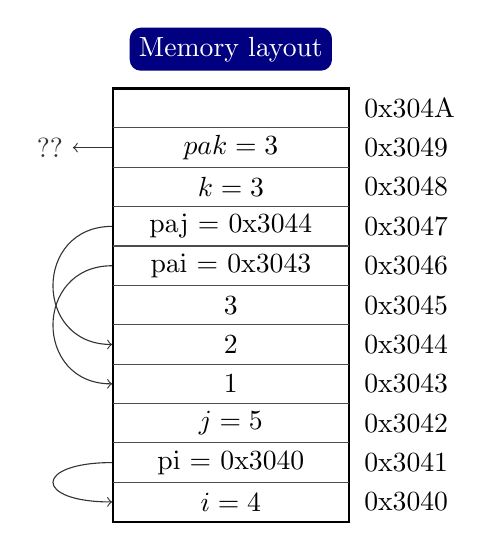
\begin{tikzpicture}
        \memorystack[size x=3cm,word size=1,nb blocks=11]
        \onslide<2-> {\memorypush{$i = 4$}}
        \onslide<3-> {\memorypushpointer[pi =]{1}}
        \onslide<4-> {\memorypush{$j = 5$}}
        \onslide<5-> {\memorypush{$1$}}
        \onslide<5-> {\memorypush{$2$}}
        \onslide<5-> {\memorypush{$3$}}
        \onslide<6-> {\memorypushpointer[pai =]{4}}
        \onslide<7-> {\memorypushpointer[paj =]{5}}
        \onslide<8-> {\memorypush{$k = 3$}}
        \onslide<9-> {\memorypush{$pak = 3$}}
        \onslide<9-> {\draw[\stackcolor!80,->] (stack10-1.west) -- +(-0.5cm,0)
          node [anchor=east] {??};}
      \end{tikzpicture}
    }
  \end{multicols}
\end{frame}

\begin{frame}[fragile]
  \frametitlecpp[11]{nullptr}
  \begin{block}{Finally a \cpp~NULL pointer}
    \begin{itemize}
    \item if a pointer doesn't point to anything, set it to \mintinline{cpp}{nullptr}
    \item works like 0 or NULL in standard cases
    \item triggers compilation error when mapped to integer
    \end{itemize}
  \end{block}
  \pause
  \begin{exampleblock}{Example code}
    \begin{cppcode*}{}
      void* vp = nullptr;
      int* ip = nullptr;
      int i = NULL;      // OK -> bug ?
      int i = nullptr;   // ERROR
    \end{cppcode*}
  \end{exampleblock}
\end{frame}

\begin{frame}[fragile]
  \frametitlecpp[98]{Dynamic Arrays}
  \begin{cppcode}
    #include <cstdlib>
    #include <cstring>

    int *bad;          // pointer to random address
    int *ai = nullptr; // better. Can be tested

    // allocate array of 10 ints (not initialized)
    ai = (int*) malloc(10*sizeof(int));
    // and set them to 0
    memset(ai, 0, 10*sizeof(int));

    // both in one go
    ai = (int*) calloc(10, sizeof(int));

    // release memory
    free(ai);
  \end{cppcode}
\end{frame}

\subsection[NS]{Scopes / namespaces}

\begin{frame}[fragile]
  \frametitlecpp[98]{Scope}
  \begin{block}{Definition}
    Portion of the source code where a given name is valid \\
    Typically :
    \begin{itemize}
    \item simple block of code, within \mintinline{cpp}{{}}
    \item function, class, namespace
    \item translation unit for global declarations
    \end{itemize}
  \end{block}
  \begin{exampleblock}{Example}
    \begin{cppcode*}{}
      { int a;
        { int b;
        } // end of b scope
      } // end of a scope
    \end{cppcode*}
  \end{exampleblock}
\end{frame}

\Scontents*[store-cmd=code_scopes]{
int a = 1;
{
  int b[4];
  b[0] = a;
}
// Doesn't compile:
// b[1] = a + 1;
}
\begin{frame}[fragile]
  \frametitlecpp[98]{Scope and lifetime of resources}
  \begin{block}{Resource life time}
    \begin{itemize}
      \item Resources are allocated when declared
      \item Resources are freed at the end of a scope
      \item Good practice: initialise resources when allocating!
    \end{itemize}
  \end{block}
  \begin{multicols}{2}
    \begin{overprint}[\columnwidth]
    \onslide<1>
    \highlightCppCode{1}{code_scopes}
    \onslide<2>
    \highlightCppCode{3}{code_scopes}
    \onslide<3>
    \highlightCppCode{4}{code_scopes}
    \onslide<4>
    \highlightCppCode{7}{code_scopes}
    \end{overprint}

    \columnbreak

    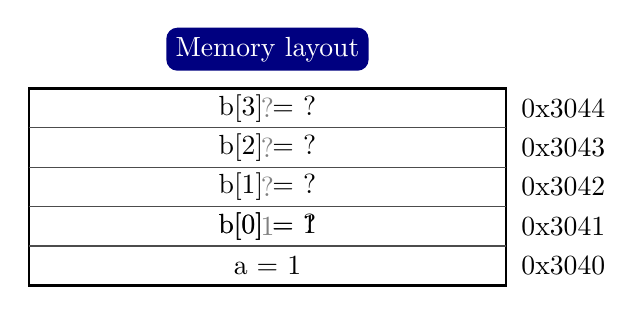
\begin{tikzpicture}
      \memorystack[word size=1, nb blocks=5, size x = 0.5\columnwidth]
      \onslide<1-> {
        \memorypush{a = 1}
      }
      \onslide<2>{
        \memorypush{b[0] = ?}
      }
      \memorygoto{2}
      \onslide<3>{
        \memorypush{b[0] = 1}
      }
      \memorygoto{3}
      \onslide<2-3>{
        \memorypush{b[1] = ?}
        \memorypush{b[2] = ?}
        \memorypush{b[3] = ?}
      }

      \memorygoto{2}
      \onslide<4>{
        \memorypush{\color{gray} 1}
        \memorypush{\color{gray} ?}
        \memorypush{\color{gray} ?}
        \memorypush{\color{gray} ?}
        }

    \end{tikzpicture}

  \end{multicols}
\end{frame}

\begin{frame}[fragile]
  \frametitlecpp[98]{Namespaces}
  \begin{itemize}
  \item Namespaces allow to segment your code to avoid name clashes
  \item They can be embedded to create hierarchies (separator is '::')
  \end{itemize}
  \begin{multicols}{2}
    \begin{cppcode*}{gobble=2}
      int a;
      namespace n {
        int a;   // no clash
      }
      namespace p {
        int a;   // no clash
        namespace inner {
          int a; // no clash
        }
      }
      int f() {
        n::a = 2;
      }
    \end{cppcode*}
    \columnbreak
    \begin{cppcode*}{gobble=2,firstnumber=14}
      namespace p {
        int f() {
          p::a = 2;
          a = 2;  //same as above
          p::inner::a = 4;
          inner::a = 4;
          n::a = 5;
        }
      }
      using namespace p::inner;
      int g() {
        a = 3; // using p::inner
      }
  \end{cppcode*}
  \end{multicols}
\end{frame}

\begin{frame}[fragile]
  \frametitlecpp[17]{Nested namespaces}
  Easier way to declare nested namespaces
  \begin{alertblock}{\cpp14}
    \begin{cppcode*}{}
      namespace A {
        namespace B {
          namespace C {
            //...
          }
        }
      }
    \end{cppcode*}
  \end{alertblock}
  \begin{exampleblock}{\cpp17}
    \begin{cppcode*}{}
      namespace A::B::C {
        //...
      }
    \end{cppcode*}
  \end{exampleblock}
\end{frame}

\begin{frame}[fragile]
  \frametitlecpp[98]{Anonymous namespaces}
  \begin{exampleblock}{A namespace without a name !}
    \begin{cppcode*}{}
      namespace {
        int localVar;
      }
    \end{cppcode*}
  \end{exampleblock}
  \begin{block}{Purpose}
    \begin{itemize}
    \item groups a number of declarations
    \item visible in the current translation unit
    \item but not reusable outside
    \item allows much better compiler optimizations and checking
      \begin{itemize}
      \item e.g. unused function warning
      \item context dependent optimizations
      \end{itemize}
    \end{itemize}
  \end{block}
  \begin{alertblock}{Deprecates static}
    \begin{cppcode*}{gobble=2}
      static int localVar; // equivalent C code
    \end{cppcode*}
  \end{alertblock}
\end{frame}

\subsection[Class/Enum]{Class and enum types}

\begin{frame}[fragile]
  \frametitlecpp[98]{struct}
  \begin{mdframed}[style=simplebox]
    \center ``members'' grouped together under one name
  \end{mdframed}
  \begin{multicols}{2}
    \begin{cppcode*}{gobble=2}
      struct Individual {
        unsigned char age;
        float weight;
      };

      Individual student;
      student.age = 25;
      student.weight = 78.5f;

      Individual teacher = {
        45, 67.0f
      };
    \end{cppcode*}
    \columnbreak
    \begin{cppcode*}{gobble=2,firstnumber=14}
      Individual *ptr = &student;
      ptr->age = 25;
      // same as: (*ptr).age = 25;
    \end{cppcode*}
    \pause
    \vfill
    \hspace{-1.5cm}
    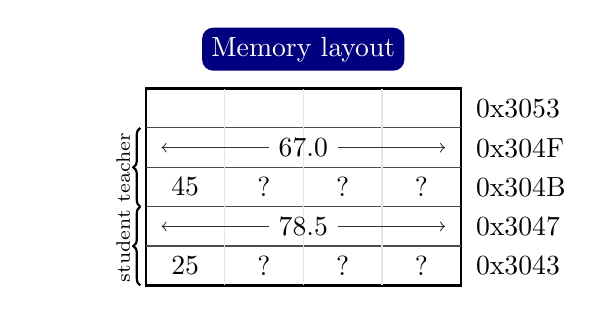
\begin{tikzpicture}
      \memorystack[nb blocks=5]
      \onslide<3-> {
        \memorypush{25,?,?,?}
        \memorypushwidevalue{78.5}
        \memorystruct{1}{2}{\scriptsize student}
      }
      \onslide<4-> {
        \memorypush{45,?,?,?}
        \memorypushwidevalue{67.0}
        \memorystruct{3}{4}{\scriptsize teacher}
      }
    \end{tikzpicture}
    \vfill \null
  \end{multicols}
\end{frame}

\begin{frame}[fragile]
  \frametitlecpp[98]{union}
  \begin{mdframed}[style=simplebox]
    \center ``members'' packed together at same memory location
  \end{mdframed}
  \begin{multicols}{2}
    \begin{cppcode*}{gobble=2}
      union Duration {
        int seconds;
        short hours;
        char days;
      };
      Duration d1, d2, d3;
      d1.seconds = 259200;
      d2.hours = 72;
      d3.days = 3;
      d1.days = 3; // d1.seconds overwritten
      int a = d1.seconds; // d1.seconds is garbage
    \end{cppcode*}
    \pause
    \columnbreak
    \null \vfill
    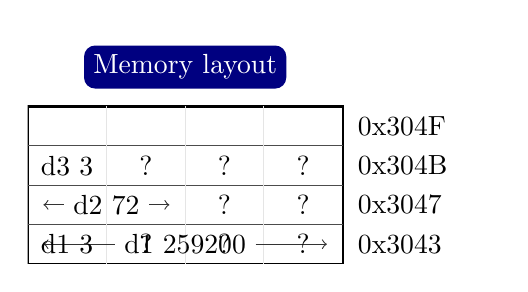
\begin{tikzpicture}
      \clip (0,0) rectangle (6cm, 3cm);
      \memorystack[word size=4,nb blocks=4]
      \visible<3-5>{\memorypushwidevalue{d1 259200}}
      \onslide<4->{\memorypushhalfvalue{d2 72}}
      \memorygoto{2}
      \onslide<4->{\memorypush{,,?,?}}
      \onslide<5->{\memorypush{d3 3,?,?,?}}
      \memorygoto{1}
      \onslide<6->{\memorypush{d1 3,?,?,?}}
    \end{tikzpicture}
    \vfill \null
  \end{multicols}
  \onslide<7->{
  \begin{alertblock}{}
    Starting with \cpp17: prefer \mintinline{cpp}{std::variant}
  \end{alertblock}
  }
\end{frame}

\begin{frame}[fragile]
  \frametitlecpp[98]{Enums}
  \begin{block}{}
    \begin{itemize}
        \item use to declare a list of related constants (enumerators)
        \item has an underlying integral type
        \item enumerator names leak into enclosing scope
    \end{itemize}
  \end{block}
  \begin{multicols}{2}
    \begin{cppcode*}{gobble=2}
      enum VehicleType {

        BIKE,  // 0
        CAR,   // 1
        BUS,   // 2
      };
      VehicleType t = CAR;
    \end{cppcode*}
    \columnbreak
    \begin{cppcode*}{gobble=2}
      enum VehicleType
        : int { // C++11
        BIKE = 3,
        CAR = 5,
        BUS = 7,
      };
      VehicleType t2 = BUS;
    \end{cppcode*}
  \end{multicols}
\end{frame}

\begin{frame}[fragile]
  \frametitlecpp[11]{Scoped enumeration, aka enum class}
  \begin{block}{Same syntax as enum, with scope}
    \begin{cppcode*}{}
      enum class VehicleType { Bus, Car };
      VehicleType t = VehicleType::Car;
    \end{cppcode*}
  \end{block}
  \pause
  \begin{exampleblock}{Only advantages}
    \begin{itemize}
    \item scopes enumerator names, avoids name clashes
    \item strong typing, no automatic conversion to int
    \end{itemize}
    \small
    \begin{cppcode*}{}
      enum VType { Bus, Car }; enum Color { Red, Blue };
      VType t = Bus;
      if (t == Red) { /* We do enter */ }
      int a = 5 * Car; // Ok, a = 5

      enum class VT { Bus, Car }; enum class Col { Red, Blue };
      VT t = VT::Bus;
      if (t == Col::Red) { /* Compiler error */ }
      int a = t * 5;       // Compiler error
    \end{cppcode*}
  \end{exampleblock}
\end{frame}

\begin{frame}[fragile]
  \frametitlecpp[98]{More sensible example}
  \begin{multicols}{2}
    \begin{cppcode*}{gobble=2}
      enum class ShapeType {
        Circle,
        Rectangle
      };

      struct Rectangle {
        float width;
        float height;
      };
    \end{cppcode*}
    \columnbreak
    \pause
    \begin{cppcode*}{gobble=2,firstnumber=10}
      struct Shape {
        ShapeType type;
        union {
          float radius;
          Rectangle rect;
        };
      };
    \end{cppcode*}
  \end{multicols}
  \pause
  \begin{multicols}{2}
    \begin{cppcode*}{gobble=2,firstnumber=17}
      Shape s;
      s.type =
        ShapeType::Circle;
      s.radius = 3.4;

    \end{cppcode*}
    \columnbreak
    \begin{cppcode*}{gobble=2,firstnumber=20}
      Shape t;
      t.type =
        Shapetype::Rectangle;
      t.rect.width = 3;
      t.rect.height = 4;
    \end{cppcode*}
  \end{multicols}
\end{frame}

\begin{frame}[fragile]
  \frametitle{typedef and using \hfill \cpp98 / \cpp11}
  Used to create type aliases
  \begin{alertblock}{\cpp98}
    \begin{cppcode*}{gobble=2}
      typedef uint64_t myint;
      myint toto = 17;
      typedef int pos[3];
    \end{cppcode*}
  \end{alertblock}
  \begin{exampleblock}{\cpp11}
    \begin{cppcode*}{gobble=2}
      using myint = uint64_t;
      myint toto = 17;
      using pos = int[3];

      template <typename T> using myvec = std::vector<T>;
      myvec<int> titi;
    \end{cppcode*}
  \end{exampleblock}
\end{frame}

\subsection[Refs]{References}

\begin{frame}[fragile]
  \frametitlecpp[98]{References}
  \begin{block}{References}
    \begin{itemize}
      \item References allow for direct access to another object
      \item They can be used as shortcuts / better readability
      \item They can be declared \cppinline{const} to allow only read access
    \end{itemize}
  \end{block}

  \begin{exampleblock}{Example:}
    \begin{cppcode*}{}
      int i = 2;
      int &iref = i; // access to i
      iref = 3;      // i is now 3

      // const reference to a member:
      struct A { int x; int y; } a;
      const int &x = a.x; // direct read access to A's x
      x = 4;              // doesn't compile
      a.x = 4;            // fine
    \end{cppcode*}
  \end{exampleblock}
\end{frame}

\begin{frame}[fragile]
  \frametitlecpp[98]{Pointers vs References}
  \begin{block}{Specificities of reference}
    \begin{itemize}
    \item Natural syntax
    \item Cannot be \cppinline{nullptr}
    \item Must be assigned when defined, cannot be reassigned
    \item References to temporary objects must be \cppinline{const}
    \end{itemize}
  \end{block}
  \begin{block}{Advantages of pointers}
    \begin{itemize}
    \item Can be \cppinline{nullptr}
    \item Can be initialized after declaration, can be reassigned
    \end{itemize}
  \end{block}
  \pause
  \begin{goodpractice}{References}
    \begin{itemize}
      \item Prefer using references instead of pointers
      \item Mark references \cppinline{const} to prevent modification
    \end{itemize}
  \end{goodpractice}
\end{frame}

\subsection[$f()$]{Functions}

\begin{frame}[fragile]
  \frametitlecpp[98]{Functions}
  \begin{multicols}{2}
    \begin{cppcode*}{gobble=2}
      // with return type
      int square(int a) {
        return a * a;
      }

      // multiple parameters
      int mult(int a,
               int b) {
        return a * b;
      }
    \end{cppcode*}
    \columnbreak
    \begin{cppcode*}{gobble=2,firstnumber=11}
      // no return
      void log(char* msg) {
        std::cout << msg;
      }

      // no parameter
      void hello() {
      	std::cout << "Hello World";
      }
    \end{cppcode*}
  \end{multicols}
\end{frame}

\begin{frame}[fragile]
  \frametitlecpp[98]{Function default arguments}
  \begin{multicols}{2}
    \begin{cppcode*}{gobble=2}
      // must be the trailing
      // argument
      int add(int a,
              int b = 2) {
        return a + b;
      }
      // add(1) == 3
      // add(3,4) == 7

    \end{cppcode*}
    \columnbreak
    \begin{cppcode*}{gobble=2,firstnumber=11}
      // multiple default
      // arguments are possible
      int add(int a = 2,
              int b = 2) {
        return a + b;
      }
      // add() == 4
      // add(3) == 5
    \end{cppcode*}
  \end{multicols}
\end{frame}


\Scontents*[store-cmd=code_bigStruct]{
struct BigStruct {...};
BigStruct s;

// parameter by value
void printBS(BigStruct p) {
  ...
}
printBS(s); // copy

// parameter by reference
void printBSp(BigStruct &q) {
  ...
}
printBSp(s); // no copy
}
\begin{frame}[fragile]
  \frametitlecpp[98]{Functions: parameters are passed by value}
  \begin{multicols}{2}
    \begin{overprint}[\columnwidth]
      \onslide<1-2>
      \highlightCppCode{2}{code_bigStruct}
      \onslide<3>
      \highlightCppCode{5,8}{code_bigStruct}
      \onslide<4->
      \highlightCppCode{11,14}{code_bigStruct}
    \end{overprint}
    \columnbreak
    \null \vfill
    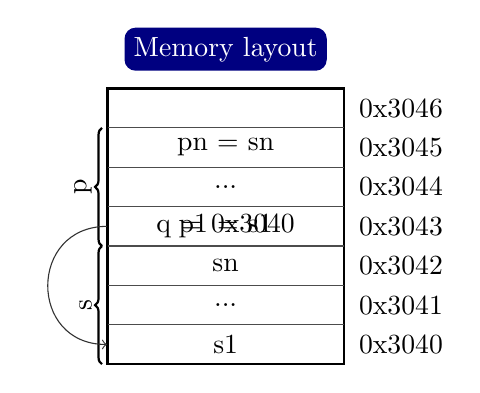
\begin{tikzpicture}
      \memorystack[word size=1, nb blocks=7, size x=3cm]
      \onslide<2-> {
        \memorypush{s1}
        \memorypush{...}
        \memorypush{sn}
        \memorystruct{1}{3}{s}
      }
      \onslide<3> {
        \memorypush{p1 = s1}
        \memorypush{...}
        \memorypush{pn = sn}
        \memorystruct{4}{6}{p}
      }
      \memorygoto{4}
      \onslide<4> {
        \memorypushpointer[q =]{1}
      }
    \end{tikzpicture}
    \vfill \null
  \end{multicols}
\end{frame}

\Scontents*[store-cmd=code_smallStruct]{
struct SmallStruct {int a;};
SmallStruct s = {1};

void changeSS(SmallStruct p) {
  p.a = 2;
}
changeSS(s);
// s.a == 1

void changeSS2(SmallStruct &q) {
  q.a = 2;
}
changeSS2(s);
// s.a == 2
}
\begin{frame}[fragile]
  \frametitlecpp[98]{Functions: pass by value or reference?}
  \begin{multicols}{2}
    \begin{overprint}[\columnwidth]
      \onslide<1>
      \highlightCppCode{}{code_smallStruct}
      \onslide<2>
      \highlightCppCode{2}{code_smallStruct}
      \onslide<3>
      \highlightCppCode{4,7}{code_smallStruct}
      \onslide<4>
      \highlightCppCode{5}{code_smallStruct}
      \onslide<5>
      \highlightCppCode{8}{code_smallStruct}
      \onslide<6>
      \highlightCppCode{10,13}{code_smallStruct}
      \onslide<7>
      \highlightCppCode{11}{code_smallStruct}
      \onslide<8>
      \highlightCppCode{14}{code_smallStruct}
    \end{overprint}
    \columnbreak
    \null \vfill
    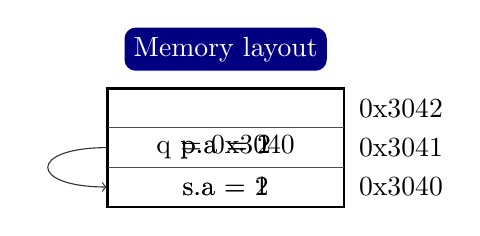
\begin{tikzpicture}
      \memorystack[word size=1, nb blocks=3, size x=3cm]
      \onslide<2-6> {
        \memorypush{s.a = 1}
      }
      \memorygoto{1}
      \onslide<7-> {
        \memorypush{s.a = 2}
      }

      \memorygoto{2}
      \onslide<3> {
        \memorypush{p.a = 1}
      }
      \memorygoto{2}
      \onslide<4> {
        \memorypush{p.a = 2}
      }
      \memorygoto{2}
      \onslide<6-7> {
        \memorypushpointer[q =]{1}
      }
      \end{tikzpicture}
    \vfill \null
  \end{multicols}
\end{frame}

\begin{frame}[fragile]
  \frametitlecpp[98]{Pass by value, reference or pointer}
  \begin{block}{Different ways to pass arguments to a function}
    \begin{itemize}
    \item by default, arguments are passed by value (= copy) \\
          good for small types, e.g.\ numbers
    \item prefer references for mandatory parameters to avoid copies
    \item use pointers for optional parameters to allow \mintinline{cpp}{nullptr}
    \item use \mintinline{cpp}{const} for safety and readability whenever possible
    \end{itemize}
  \end{block}
  \pause
  \begin{block}{Syntax}
    \begin{cppcode*}{escapeinside=||}
struct T {...}; T a;
void f(T value);           f(a);      // by value
void fRef(const T &value); fRef(a);   // by reference
void fPtr(const T *value); fPtr(|{\setlength{\fboxsep}{0pt}\color{gray}\colorbox{yellow}{\textsc{&}}}|a);  // by pointer
void fWrite(T &value);     fWrite(a); // non-const ref
    \end{cppcode*}
  \end{block}
\end{frame}

\begin{frame}[fragile]
  \frametitlecpp[98]{Functions}
  \begin{alertblock}{Exercise}
    Familiarise yourself with pass by value / pass by reference.
    \begin{itemize}
      \item go to \texttt{code/functions}
      \item Look at \texttt{functions.cpp}
      \item Compile it (\texttt{make}) and run the program (\texttt{./functions})
      \item Work on the tasks that you find in \texttt{functions.cpp}
    \end{itemize}
  \end{alertblock}
\end{frame}

\begin{frame}[fragile]
  \frametitlecpp[98]{Functions: good practices}
  \begin{onlyenv}<1>
    \begin{block}{Ensure good readability/maintainability:}
      \begin{itemize}
        \item Keep functions short
        \item Do one logical thing (single-responsibility principle)
        \item Use expressive names
        \item Document non-trivial functions
      \end{itemize}
    \end{block}
    \begin{exampleblock}{Example: Good}
      \begin{cppcode*}{gobble=2}
        /// Count number of dilepton events in data.
        /// \param d Dataset to search.
        unsigned int countDileptons(Data d) {
          selectEventsWithMuons(d);
          selectEventsWithElectrons(d);
          return d.size();
        }
      \end{cppcode*}
    \end{exampleblock}
  \end{onlyenv}
  \begin{onlyenv}<2->
    \begin{alertblock}{Example: don't! Everything in one long function}
      \begin{multicols}{2}
        \begin{cppcode*}{gobble=6}
          unsigned int runJob() {
            // Step 1: data
            Data data;
            data.resize(123456);
            data.fill(...);

            // Step 2: muons
            for (....) {
              if (...) {
                data.erase(...);
              }
            }
            // Step 3: electrons
            for (....) {
        \end{cppcode*}
        \columnbreak
        \begin{cppcode*}{gobble=6,firstnumber=last}
              if (...) {
                data.erase(...);
              }
            }

            // Step 4: dileptons
            int counter = 0;
            for (....) {
              if (...) {
                counter++;
              }
            }

            return counter;
          }
        \end{cppcode*}
      \end{multicols}
    \end{alertblock}
  \end{onlyenv}
\end{frame}

\subsection[Op]{Operators}

\begin{frame}[fragile]
  \frametitlecpp[98]{Operators(1)}
  \begin{block}{Binary and Assignment Operators}
    \begin{cppcode*}{}
      int i = 1 + 4 - 2;  // 3
      i *= 3;             // 9, short for: i = i * 3;
      i /= 2;             // 4
      i = 23 % i;         // modulo => 3
    \end{cppcode*}
  \end{block}
  \pause
  \begin{block}{Increment / Decrement Operators \uncover<3->{\hfill \alert{\bf Use wisely}}}
    \begin{cppcode*}{}
      int i = 0; i++; // i = 1
      int j = ++i;    // i = 2, j = 2
      int k = i++;    // i = 3, k = 2
      int l = --i;    // i = 2, l = 2
      int m = i--;    // i = 1, m = 2
    \end{cppcode*}
  \end{block}
\end{frame}

\begin{frame}[fragile]
  \frametitlecpp[98]{Operators(2)}
  \begin{block}{Bitwise and Assignment Operators}
    \begin{cppcode*}{}
      unsigned i = 0xee & 0x55;  // 0x44
      i |= 0xee;                 // 0xee
      i ^= 0x55;                 // 0xbb
      unsigned j = ~0xee;        // 0xffffff11
      unsigned k = 0x1f << 3;    // 0xf8
      unsigned l = 0x1f >> 2;    // 0x7
    \end{cppcode*}
  \end{block}
  \pause
  \begin{block}{Logical Operators}
    \begin{cppcode*}{}
      bool a = true;
      bool b = false;
      bool c = a && b;    // false
      bool d = a || b;    // true
      bool e = !d;        // false
    \end{cppcode*}
  \end{block}
\end{frame}

\begin{frame}[fragile]
  \frametitlecpp[98]{Operators(3)}
  \begin{block}{Comparison Operators}
    \begin{cppcode*}{}
      bool a = (3 == 3);  // true
      bool b = (3 != 3);  // false
      bool c = (4 <  4);  // false
      bool d = (4 <= 4);  // true
      bool e = (4 >  4);  // false
      bool f = (4 >= 4);  // true
      auto g = (5 <=> 5); // C++20 (later)
    \end{cppcode*}
  \end{block}
  \pause
  \begin{block}{Precedences \uncover<3->{\hfill \alert{\bf Avoid}\uncover<4->{\color{green} \bf\ - use parentheses}}}
    \begin{cppcode*}{linenos=false}
      c &= 1+(++b)|(a--)*4%5^7; // ???
    \end{cppcode*}
    Details can be found on {\color{blue!50!white} \href{https://en.cppreference.com/w/cpp/language/operator_precedence}{cppreference}}
  \end{block}
\end{frame}

\subsection[Control]{Control structures}

\begin{frame}[fragile]
  \frametitlecpp[98]{Control structures: if}
  \begin{block}{if syntax}
    \begin{cppcode*}{}
      if (condition1) {
        Statement1; Statement2;
      } else if (condition2)
        OnlyOneStatement;
      else {
        Statement3;
        Statement4;
      }
    \end{cppcode*}
    \begin{itemize}
      \item The \mintinline{cpp}{else} and \mintinline{cpp}{else if} clauses are optional
      \item The \mintinline{cpp}{else if} clause can be repeated
      \item Braces are optional if there is a single statement
    \end{itemize}
  \end{block}
\end{frame}

\begin{frame}[fragile]
  \frametitlecpp[98]{Control structures: if}
  \begin{exampleblock}{Practical example}
    \begin{cppcode*}{}
      int collatz(int a) {
        if (a <= 0) {
          std::cout << "not supported";
          return 0;
        } else if (a == 1) {
          return 1;
        } else if (a%2 == 0) {
          return collatz(a/2);
        } else {
          return collatz(3*a+1);
        }
      }
    \end{cppcode*}
  \end{exampleblock}
\end{frame}

\begin{frame}[fragile]
  \frametitlecpp[98]{Control structures: conditional operator}
  \begin{block}{Syntax}
    \begin{cppcode*}{linenos=false}
      test ? expression1 : expression2;
    \end{cppcode*}
    \vspace{-0.2cm}
    \begin{itemize}
      \item If test is \mintinline{cpp}{true} expression1 is returned
      \item Else, expression2 is returned
    \end{itemize}
  \end{block}
  \pause
  \begin{exampleblock}{Practical example}
    \begin{cppcode*}{}
      int collatz(int a) {
        return a==1 ? 1 : collatz(a%2==0 ? a/2 : 3*a+1);
      }
    \end{cppcode*}
  \end{exampleblock}
  \pause
  \begin{alertblock}{Do not abuse it}
    \begin{itemize}
      \item Explicit \mintinline{cpp}{if}s are generally easier to read
      \item Use the ternary operator with short conditions and expressions
      \item Avoid nesting
    \end{itemize}
  \end{alertblock}
\end{frame}

\begin{frame}[fragile]
  \frametitlecpp[98]{Control structures: switch}
  \begin{block}{Syntax}
    \begin{cppcode*}{gobble=2}
      switch(identifier) {
        case c1 : statements1; break;
        case c2 : statements2; break;
        case c3 : statements3; break;
        ...
        default : instructiond; break;
      }
    \end{cppcode*}
    \begin{itemize}
      \item The \mintinline{cpp}{break} statement is not mandatory but...
      \item Cases are entry points, not independent pieces
      \item Execution falls through to the next case without a \mintinline{cpp}{break}!
      \item The \mintinline{cpp}{default} case may be omitted
    \end{itemize}
  \end{block}
  \pause
  \begin{alertblock}{Use break}
    Avoid \mintinline{cpp}{switch} statements with fall-through cases
  \end{alertblock}
\end{frame}

\begin{frame}[fragile]
  \frametitlecpp[98]{Control structures: switch}
  \begin{exampleblock}{Practical example}
    \begin{cppcode*}{}
      enum class Lang { French, German, English, Other };
      ...
      switch (language) {
      case Lang::French:
        std::cout << "Bonjour";
        break;
       case Lang::German:
        std::cout << "Guten Tag";
        break;
      case Lang::English:
        std::cout << "Good morning";
        break;
      default:
        std::cout << "I do not speak your language";
      }
    \end{cppcode*}
  \end{exampleblock}
\end{frame}

\AtBeginEnvironment{minted}{\renewcommand{\fcolorbox}[4][]{#4}}

\begin{frame}[fragile]
  \frametitlecpp[17]{\texttt{[[fallthrough]]} attribute}
  \begin{block}{New compiler warning}
    Since \cpp17, compilers are encouraged to warn on fall-through
  \end{block}
  \begin{exampleblock}{\cpp17}
    \begin{cppcode*}{}
      switch (c) {
        case 'a':
          f();    // Warning emitted
        case 'b': // Warning emitted
        case 'c':
          g();
          [[fallthrough]]; // Warning suppressed
        case 'd':
          h();
      }
    \end{cppcode*}
  \end{exampleblock}
\end{frame}

\begin{frame}[fragile]
  \frametitlecpp[17]{Init-statements for if and switch}
  \begin{block}{}
    Allows to limit variable scope in \mintinline{cpp}{if} and \mintinline{cpp}{switch} statements
  \end{block}
  \begin{exampleblock}{\cpp17}
    \begin{cppcode*}{}
      if (Value val = GetValue(); condition(val)) {
        f(val);
      } else {
        g(val);
      }
      h(val); // compile error
    \end{cppcode*}
  \end{exampleblock}
  \pause
  \begin{alertblock}{\cpp98}
    Don't confuse with a variable declaration as condition:
    \begin{cppcode*}{firstnumber=7}
      if (Value* val = GetValuePtr())
        f(*val);
    \end{cppcode*}
  \end{alertblock}
\end{frame}

\begin{frame}[fragile]
  \frametitlecpp[98]{Control structures: for loop}
  \begin{block}{for loop syntax}
    \begin{cppcode*}{}
      for(initializations; condition; increments) {
        statements;
      }
    \end{cppcode*}
    \vspace{-0.2cm}
    \begin{itemize}
      \item Initializations and increments are comma separated
      \item Initializations can contain declarations
      \item Braces are optional if loop body is a single statement
    \end{itemize}
  \end{block}
  \pause
  \begin{exampleblock}{Practical example}
    \begin{cppcode*}{firstnumber=4}
      for(int i = 0, j = 0 ; i < 10 ; i++, j = i*i) {
        std::cout << i << "^2 is " << j << '\n';
      }
    \end{cppcode*}
  \end{exampleblock}
  \pause
  \begin{goodpracticeWithShortcut}{Don't abuse the \texttt{for} syntax}{\texttt{for} syntax}
    \begin{itemize}
      \item The \mintinline{cpp}{for} loop head should fit in 1-3 lines
    \end{itemize}
  \end{goodpracticeWithShortcut}
\end{frame}

\begin{frame}[fragile]
  \frametitlecpp[11]{Range-based loops}
  \begin{block}{Reason of being}
    \begin{itemize}
    \item Simplifies loops over ``ranges'' tremendously
    \item Especially with STL containers
    \end{itemize}
  \end{block}
  \begin{block}{Syntax}
    \begin{cppcode*}{}
      for ( type iteration_variable : range ) {
        // body using iteration_variable
      }
    \end{cppcode*}
  \end{block}
  \begin{exampleblock}{Example code}
    \begin{cppcode*}{firstnumber=4}
      int v[4] = {1,2,3,4};
      int sum = 0;
      for (int a : v) { sum += a; }
    \end{cppcode*}
  \end{exampleblock}
\end{frame}

\begin{frame}[fragile]
  \frametitlecpp[20]{Init-statements for range-based loops}
  \begin{block}{}
    Allows to limit variable scope in range-based loops
  \end{block}
  \begin{alertblock}{\cpp17}
    \begin{cppcode*}{}
      std::array data = {"hello", ",", "world"};
      std::size_t i = 0;
      for (auto& d : data) {
        std::cout << i++ << ' ' << d << '\n';
      }
    \end{cppcode*}
  \end{alertblock}
  \begin{exampleblock}{\cpp20}
    \begin{cppcode*}{firstnumber=6}
      std::array data = {"hello", ",", "world"};
      for (std::size_t i = 0; auto& d : data) {
        std::cout << i++ << ' ' << d << '\n';
      }
    \end{cppcode*}
  \end{exampleblock}
\end{frame}

\begin{frame}[fragile]
  \frametitlecpp[98]{Control structures: while loop}
  \begin{block}{while loop syntax}
    \begin{cppcode*}{}
      while(condition) {
        statements;
      }
      do {
        statements;
      } while(condition);
    \end{cppcode*}
    \begin{itemize}
      \item Braces are optional if the body is a single statement
    \end{itemize}
  \end{block}
  \pause
  \begin{alertblock}{Bad example}
    \begin{cppcode*}{}
      while (n != 1)
        if (0 == n%2) n /= 2;
        else n = 3 * n + 1;
    \end{cppcode*}
  \end{alertblock}
\end{frame}

\begin{frame}[fragile]
  \frametitlecpp[98]{Control structures: jump statements}
  \begin{block}{}
    \begin{description}
    \item[break] Exits the loop and continues after it
    \item[continue] Goes immediately to next loop iteration
    \item[return] Exits the current function
    \item[goto] Can jump anywhere inside a function, avoid!
    \end{description}
  \end{block}
  \pause
  \begin{alertblock}{Bad example}
    \begin{cppcode*}{}
      while (1) {
        if (n == 1) break;
        if (0 == n%2) {
          std::cout << n << '\n';
          n /= 2;
          continue;
        }
        n = 3 * n + 1;
      }
    \end{cppcode*}
  \end{alertblock}
\end{frame}

\begin{frame}[fragile]
  \frametitlecpp[11]{Control structures}
  \begin{exerciseWithShortcut}{Control structures}{Control structs}
    Familiarise yourself with different kinds of control structures. Re-implement them in different ways.
    \begin{itemize}
      \item Go to \texttt{code/control}
      \item Look at \texttt{control.cpp}
      \item Compile it (\texttt{make}) and run the program (\texttt{./control})
      \item Work on the tasks that you find in \texttt{README.md}
    \end{itemize}
  \end{exerciseWithShortcut}
\end{frame}

\subsection[.h]{Headers and interfaces}

\begin{frame}[fragile]
  \frametitlecpp[98]{Headers and interfaces}
  \begin{block}{Interface}
    Set of declarations defining some functionality
    \begin{itemize}
    \item Put in a so-called ``header file''
    \item The implementation exists somewhere else
    \end{itemize}
  \end{block}
  \begin{block}{Header: hello.hpp}
    \begin{cppcode*}{linenos=false}
      void printHello();
    \end{cppcode*}
  \end{block}
  \begin{block}{Usage: myfile.cpp}
    \begin{cppcode*}{}
      #include "hello.hpp"
      int main() {
        printHello();
      }
    \end{cppcode*}
  \end{block}
\end{frame}

\begin{frame}[fragile]
  \frametitlecpp[98]{Preprocessor}
  \begin{cppcode}
    // file inclusion
    #include "hello.hpp"
    // macro constants and function-style macros
    #define MY_GOLDEN_NUMBER 1746
    #define CHECK_GOLDEN(x) if ((x) != MY_GOLDEN_NUMBER) \
      std::cerr << #x " was not the golden number\n";
    // compile time or platform specific configuration
    #if defined(USE64BITS) || defined(__GNUG__)
      using myint = std::uint64_t;
    #elif
      using myint = std::uint32_t;
    #endif
  \end{cppcode}
  \pause
  \begin{goodpracticeWithShortcut}{Use preprocessor only in very restricted cases}{preprocessor}
    \begin{itemize}
      \item Conditional inclusion of headers
      \item Customization for specific compilers/platforms
    \end{itemize}
  \end{goodpracticeWithShortcut}
\end{frame}

\begin{frame}[fragile]
  \frametitlecpp[98]{Header include guards}
  \begin{block}{Problem: redefinition by accident}
    \begin{itemize}
      \item Headers may define new names (e.g.\ types)
      \item Multiple (transitive) inclusions of a header would define those names multiple times, which is a compile error
      \item Solution: guard the content of your headers!
    \end{itemize}
  \end{block}
  \begin{block}{Include guards}
    \begin{cppcode*}{}
      #ifndef MY_HEADER_INCLUDED
      #define MY_HEADER_INCLUDED
      ... // header file content
      #endif
    \end{cppcode*}
  \end{block}
  \begin{block}{Pragma once (non-standard)}
    \begin{cppcode*}{}
      #pragma once
      ... // header file content
    \end{cppcode*}
  \end{block}
\end{frame}

\subsection[auto]{Auto keyword}

\begin{frame}[fragile]
  \frametitlecpp[11]{Auto keyword}
  \begin{block}{Reason of being}
    \begin{itemize}
    \item Many type declarations are redundant
    \item They are often a source for compiler warnings and errors
    \item Using auto prevents unwanted/unnecessary type conversions
    \end{itemize}
    \begin{cppcode*}{}
      std::vector<int> v;
      float a = v[3];    // conversion intended?
      int b = v.size();  // bug? unsigned to signed
    \end{cppcode*}
  \end{block}
  \pause
  \begin{block}{Practical usage}
    \begin{cppcode*}{}
      std::vector<int> v;
      auto a = v[3];
      const auto b = v.size(); // std::size_t
      int sum{0};
      for (auto n : v) { sum += n; }
    \end{cppcode*}
  \end{block}
\end{frame}

\begin{frame}[fragile]
  \frametitlecpp[98]{Loops, references, auto}
  \begin{exerciseWithShortcut}{Loops, references, auto}{Loops, refs, auto}
    Familiarise yourself with range-based for loops and references
    \begin{itemize}
      \item Go to \texttt{exercises/loopsRefsAuto}
      \item Look at \texttt{loopsRefsAuto.cpp}
      \item Compile it (\texttt{make}) and run the program (\texttt{./loopsRefsAuto})
      \item Work on the tasks that you find in \texttt{loopsRefsAuto.cpp}
    \end{itemize}
  \end{exerciseWithShortcut}
\end{frame}


%\includeonlyframes{current}

\subsection{Objects and Classes}

\begin{frame}[fragile]
  \frametitle{What are classes and objects}
  \begin{block}{Classes}
    structs on steroids
    \begin{itemize}
    \item with inheritance
    \item with associated methods
    \end{itemize}
  \end{block}
  \begin{block}{Objects}
    instances of classes
  \end{block}
  \begin{block}{Encapsulates a concept}
    \begin{itemize}
    \item shows an interface
    \item provides its implementation
      \begin{itemize}
      \item status, properties
      \item possible interactions
      \item construction and destruction
      \end{itemize}    
    \end{itemize}    
  \end{block}
\end{frame}


\begin{frame}[fragile]
  \frametitle{My First Class}
  \begin{multicols}{2}
    \begin{cppcode*}{gobble=6}
      struct MyFirstClass {
        int a;
        void squareA() {
          a *= a;
        };
      };

      MyFirstClass myObj;
      myObj.a = 2;

      // let's square a
      myObj.squareA();
    \end{cppcode*}
    \columnbreak
    \null \vfill
    \begin{tikzpicture}
      \tcbset{minted options={gobble=8}}
      \begin{CodeNode}{0,-2}{MyFirstClass}{MyFirstClass}
        int a;
        void squareA();
      \end{CodeNode}
    \end{tikzpicture}
    \vfill \null
  \end{multicols}
\end{frame}




\begin{frame}[fragile,label=current]
\xxx
  \frametitle{Static members}
  \begin{block}{Concept}
    \begin{itemize}
    \item members attached to a class rather than to an object
    \item usable with or without an instance of the class
    \item identified by the {\it static} keyword
    \end{itemize}
  \end{block}
  \begin{cppcode*}{}
    Class Text {
    public:
      static std::string upper(std::string);
    private:
      static int s_bCallsToUpper;
    }
    int Text::s_bCallsToUpper = 0;
    std::string s = "my text";
    std::string uppers = Text::upper("my text");
    // now Text::s_bCallsToUpper is 1
  \end{cppcode*}
\end{frame}

\begin{frame}[fragile,label=current]
  \frametitle{private/ public inheritance}
  /xxx
\end{frame}

\begin{frame}[fragile,label=current]
  \frametitle{static functions}
  /xxx
\end{frame}

\begin{frame}[fragile,label=current]
  \frametitle{static variable}
  /xxx
\end{frame}

\begin{frame}[fragile]
  \frametitle{Separating the interface}
  \begin{block}{Header : MyFirstClass.hpp}
    \begin{cppcode*}{linenos=false,gobble=6}
      struct MyFirstClass {
        int a;
        void squareA();
      };
    \end{cppcode*}
  \end{block}
  \begin{block}{Implementation : MyFirstClass.cpp}
    \begin{cppcode*}{linenos=false,gobble=6}
      #include "MyFirstClass.hpp"
      void MyFirstClass::squareA() {
        a *= a;
      };
    \end{cppcode*}
  \end{block}
\end{frame}

\begin{frame}[fragile]
  \frametitle{A word on namespaces}
  \begin{itemize}
  \item Namespaces allow to segment your code to avoid name clashes
  \item They can be embedded to create hierarchies (separator is '::')
  \end{itemize}
  \begin{multicols}{2}
    \begin{cppcode*}{gobble=6}
      namespace n {
        int a;
      }      
      namespace p {
        int a; // no clash
        namespace inner {
          int a; // no clash
        }
      }
      int f() {
        n::a = 2;
      }
    \end{cppcode*}
    \columnbreak
    \begin{cppcode*}{gobble=6,firstnumber=13}
      namespace p {
        int f() {
          p::a = 2;
          a = 2;  //same as above
          p::inner::a = 4;
          inner::a = 4;
          n::a = 5;
        }
      }
      using namespace p::inner;
      int g() {
        a = 3; // using p::inner
      }
  \end{cppcode*}
  \end{multicols}
\end{frame}

\begin{frame}[fragile]
  \frametitle{Implementing methods}
  \begin{block}{Standard practice}
    \begin{itemize}
    \item usually in .cpp, outside of class declaration
    \item using the class name as namespace
    \item when reference to the object is needed, use {\it this} keyword
    \end{itemize}
  \end{block}
  \begin{cppcode*}{}
    void MyFirstClass::squareA() {
      a *= a;
    };

    int MySecondClass::sum() {
      int a = 0; // do not do that !
      a += this->a;
      a += this->b;
      return a;
    };
  \end{cppcode*}
\end{frame}

\begin{frame}[fragile]
  \frametitle{Method overloading}
  \begin{block}{The rules in \cpp}
    \begin{itemize}
    \item overloading is authorized and welcome
    \item signature is part of the method identity
    \item but not the return code
    \end{itemize}
  \end{block}
  \begin{cppcode*}{}
    class MySecondClass : MyFirstClass {
    public:
      int sum();
      int sum(int c);
    }

    int MySecondClass::sum() { return a + b; };

    int MySecondClass::sum(int c) { return a + b + c; };
  \end{cppcode*}
\end{frame}

\subsection{Inheritance}

\begin{frame}[fragile]
  \frametitle{First inheritance}
  \begin{multicols}{2}
    \begin{cppcode*}{gobble=6,firstnumber=13}
      struct MySecondClass :
        MyFirstClass {
        int b;
        int sum() {
          return a + b;
        };
      };

      MySecondClass myObj2;
      myObj2.a = 2;
      myObj2.b = 5;

      myObj2.squareA();
      int i = myObj2.sum();
      // i = 9
    \end{cppcode*}
    \columnbreak
    \null \vfill
    \begin{tikzpicture}
      \tcbset{minted options={gobble=8}}
      \begin{CodeNode}{0,1.5}{MyFirstClass}
        int a;
        void squareA();
      \end{CodeNode}
      \begin{CodeNode}{0,-1.5}{MySecondClass}
        int b;
        int sum();
      \end{CodeNode}
    \draw[very thick,->] (MySecondClass)--(MyFirstClass);
    \end{tikzpicture}
    \vfill \null
  \end{multicols}
\end{frame}


\subsection{Encapsulation}

\begin{frame}[fragile]
  \frametitle{Managing access to class members}
  \begin{block}{{\it public} / {\it private} keywords}
    \begin{itemize}
      \item {\it private} : access only inside the class
      \item {\it public} : access from anywhere
      \item Default is {\it private}
      \item A {\it struct} is a {\it class} fully public
    \end{itemize}
  \end{block}
  \pause
  \begin{multicols}{2}
    \begin{cppcode*}{gobble=6}
      class MyFirstClass {
      public:
        void setA(int a);
        int getA();
        void squareA();
      private:
        int a;
      }
    \end{cppcode*}
    \columnbreak
    \begin{cppcode*}{gobble=6,firstnumber=9}
      MyFirstClass obj;
      obj.a = 5;   // error !
      obj.setA(5); // ok
      obj.squareA();
      int b = obj.getA();
    \end{cppcode*}
    \pause
    \begin{tcolorbox}[left=0mm,right=0mm,top=0mm,bottom=0mm,colback=red!5!white,colframe=red!75!black]
      This breaks MySecondClass !
    \end{tcolorbox}
  \end{multicols}
\end{frame}

\begin{frame}[fragile]
  \frametitle{Managing access to class members(2)}
  \begin{block}{Solution is {\it protected} keyword}
    Gives access to class descendant
  \end{block}
  \begin{multicols}{2}
    \begin{cppcode*}{gobble=6}
      class MyFirstClass {
      public:
        void setA(int a);
        int getA();
        void squareA();
      protected:
        int a;
      }
    \end{cppcode*}
    \columnbreak
    \begin{cppcode*}{gobble=6,firstnumber=13}
      class MySecondClass :
        MyFirstClass {
      public:
        int sum() {
          return a + b;
        };
      private:
        int b;
      }
    \end{cppcode*}
  \end{multicols}
\end{frame}


\subsection{constructors and destructors}


\begin{frame}[fragile]
  \frametitle{Class Constructors and Destructor}
  \begin{block}{Concept}
    \begin{itemize}
    \item special functions building/destroying an object
    \item a class can have several constructors
    \item the constructors have the name of the class
    \item same for the destructor with a leading $\sim$
    \end{itemize}
  \end{block}
  \begin{multicols}{2}
    \begin{cppcode*}{gobble=6}
      class MyFirstClass {
      public:
        MyFirstClass();
        MyFirstClass(int a);
        ~MyFirstClass();
        ...
      protected:
        int a;
      };
    \end{cppcode*}
    \columnbreak
    \begin{cppcode*}{gobble=6,firstnumber=10}
      // note special notation for
      // initialization of members
      MyFirstClass() : a(0) {}
      
      MyFirstClass(int a_):a(_a) {}

      ~MyFirstClass(){};
    \end{cppcode*}
  \end{multicols}
\end{frame}


\begin{frame}[fragile]
  \frametitle{Class Constructor and Destructors}
  \begin{cppcode*}{}
    class Vector {
    public:
      Vector(int n);
      ~Vector();
      void setN(int n, int value);
      int getN(int n);
    private:
      int len;
      int* data;
    }
    Vector::Vector(int n) : len(n) {
      data = (int*)malloc(n*sizeof(int));
    }
    Vector::~Vector() {
      free(data);
    }
  \end{cppcode*}
\end{frame}


\begin{frame}[fragile]
  \frametitle{Constructor and inheritance}
  \begin{cppcode*}{}
    struct MyFirstClass {
      MyFirstClass();
      MyFirstClass(int a);
    }

    struct MySecondClass : MyFirstClass {
      MySecondClass();
      MySecondClass(int b);
      MySecondClass(int a, int b);
    }

    MySecondClass() : MyFirstClass(), b(0) {};
    MySecondClass(int b_) : MyFirstClass(), b(b_) {};
    MySecondClass(int a_,
                  int b_) : MyFirstClass(a_), b(b_) {};
  \end{cppcode*}
\end{frame}

\begin{frame}[fragile]
  \frametitle{Object lifetime}
  \begin{block}{On the stack}
    \begin{itemize}
    \item object are created when declared (constructor called)
    \item object are destructed when out of scope (destructor is called)
    \end{itemize}
  \end{block}
  \begin{cppcode*}{}
    {
      MyFirstClass a; // default constructor called
      ...
    }  // destructor called

    int f() {
      MyFirstClass a(3); // constructor called
      ...
    } // destructor called
  \end{cppcode*}
\end{frame}

\begin{frame}[fragile]
  \frametitle{Object lifetime}
  \begin{block}{On the heap}
    \begin{itemize}
    \item object are created by calling {\it new} (constructor is called)
    \item object are destructed by calling {\it delete} (destructor is called)
    \end{itemize}
  \end{block}
  \begin{cppcode*}{}
    {
      // default constructor called
      MyFirstClass *a = new MyFirstClass;
      ...
      delete a; // destructor is called
    }

    int f() {
      // constructor called
      MyFirstClass *a = new MyFirstClass(3);
      ...
    } // memory leak !!!
  \end{cppcode*}
\end{frame}

\subsection{Exceptions}

\begin{frame}[fragile]
  \frametitle{Exceptions}
  \begin{block}{The concept}
    \begin{itemize}
    \item exceptional Event breaking linearity of the code
    \item will be handled in dedicated place
    \end{itemize}
  \end{block}
  \begin{block}{Pratically}
    \begin{itemize}
    \item you can throw any object with {\it throw}
    \item you handle them using {\it try ... catch} blocks
    \end{itemize}
  \end{block}
  \begin{cppcode*}{}
    try {
      if (0 == name) {
        throw std::string("Expected non empty name");
      }
      printf("%s\n", name);
    } catch (std::string e) {
      printf("empty name found\n");      
    }
  \end{cppcode*}
\end{frame}

\begin{frame}[fragile]
  \frametitle{Exceptions}
  \begin{block}{Rules}
    \begin{itemize}
    \item exception will skip all code until next {\it catch}
    \begin{itemize}
      \item still destructors are called when exiting scopes
      \item but your own cleanup may not be
    \end{itemize}
    \item {\it catch} is selective on the exception type
    \end{itemize}
  \end{block}
  \begin{multicols}{2}
    \begin{cppcode*}{fontsize=\scriptsize,gobble=6}
      class ZeroDivide {};
      
      int divide(int a, int b) {
        if (0 == b) {
          throw ZeroDivide();
        }
        return a/b;
      }
    \end{cppcode*}
    \columnbreak
    \begin{cppcode*}{fontsize=\scriptsize,gobble=6,firstnumber=9} 
      int func(char* value) {
        try {
          errno = 0;
          long l = strtol(value,0,10);
          if (errno) {
            throw string("Bad Value");
          }
          divide(100, l);
        } catch (string e) {
          printf("%s\n", e.c_str());
        } catch (ZeroDivide e2) {
          printf("Division error\n");
        }
      }
    \end{cppcode*}
  \end{multicols}
\end{frame}

\xxx throw declaration for a function
\xxx only at run time !!!

\section[More]{More \cpp features}

\subsection[const]{Constant Expressions}

\begin{frame}[fragile]
  \frametitleii{Generalized Constant Expressions}
  \begin{block}{Reason of being}
    \begin{itemize}
    \item compute constant expressions at compile time
    \item even if non trivial
    \end{itemize}
  \end{block}
  \pause
  \begin{exampleblock}{Example}
    \begin{cppcode*}{linenos=false}
      constexpr int f(int x) {
        return x > 1 ? x * f(x - 1) : 1;
      }
      int a = f(5); // now computed at compile time
    \end{cppcode*}
  \end{exampleblock}
\end{frame}

\begin{frame}[fragile]
  \frametitleii{Generalized Constant Expressions(2)}
  \begin{alertblock}{Few limitations}
    \begin{itemize}
    \item function's body cannot contain try-catch or static variables
    \item arguments should be constexpr or literals in order to benefit from compile time computation
    \end{itemize}
  \end{alertblock}
  \begin{block}{Notes}
    \begin{itemize}
    \item classes can have constexpr functions
    \item objects can be constexpr
      \begin{itemize}
      \item if the constructor of their class is
      \end{itemize}
    \item a constexpr function can also be used normally
    \end{itemize}
  \end{block}
\end{frame}

\begin{frame}[fragile]
  \frametitleii{Real life example}
  \begin{cppcode*}{linenos=true}
    constexpr float toSI(const float v, const char unit) {
      switch (unit) {
      case 'k': return 1000*v;
      case 'm': return 0.001*v;
      case 'y': return 0.9144*v;
      case 'i': return 0.0254*v;
      ...
      default: return v;
      }
    }
    constexpr float fromSI(const float v, const char unit) {
      switch (unit) {
      case 'k': return 0.001*v;
      ...
      }
    }
  \end{cppcode*}
\end{frame}

\begin{frame}[fragile]
  \frametitleii{Real life example(2)}
  \begin{cppcode*}{linenos=true}
    class DimLength {
      const float m_value;
    public:
      constexpr DimLength(const float v, const char unit):
        m_value(convertToSI(v, unit)) {
      }
      constexpr float get(const char unit) const {
        return convertFromSI(m_value, unit);
      }
    };
    constexpr DimLength km(1, 'k');
    constexpr float km_y = km.get('y');
    constexpr float km_i = km.get('i');
    std::cout << "1 km = " << km_y << " yards\n"
              << "     = " << km_i << " inches\n";
  \end{cppcode*}
\end{frame}


\subsection[auto]{Auto keyword}

\begin{frame}[fragile]
  \frametitleii{Auto keyword}
  \begin{block}{Reason of being}
    \begin{itemize}
    \item many type declarations are redundant
    \item and lead to compiler error if you mess up
    \end{itemize}
    \begin{cppcode*}{linenos=false}
      std::vector<int> v;
      int a = v[3];
      int b = v.size();  // bug ? unsigned to signed
    \end{cppcode*}
  \end{block}
  \pause
  \begin{block}{Practical usage}
    \begin{cppcode*}{linenos=false}
      std::vector<int> v;
      auto a = v[3];
      auto b = v.size();
      int sum{0};
      for (auto n : v) { sum += n; }
    \end{cppcode*}
  \end{block}
\end{frame}

\subsection[Refs]{References}

\begin{frame}[fragile]
  \frametitlegb{Value, pointers and references}
  \begin{block}{Different ways to pass arguments to a function}
    \begin{itemize}
    \item by default arguments are passed by value
    \item but pointers can be used
    \item and references are also available in \cpp11
    \end{itemize}
  \end{block}
  \begin{cppcode}
    struct T {...};
    void func   (T value);  // by value
    void funcPtr(T *value); // pointer
    void funcRef(T &value); // reference
  \end{cppcode}
\end{frame}

\begin{frame}[fragile]
  \frametitlegb{Value versus pointers/reference}
  \begin{block}{Identical to C}
    \begin{itemize}
    \item by value, a copy is created
      \begin{itemize}
        \item calling the copy constructor for objects
      \end{itemize}
    \item using pointers, the memory address of value is passed
    \item using reference, a reference to value is passed
    \end{itemize}
  \end{block}
  \begin{cppcode}
    T a;      // constructor called
  \end{cppcode}
  \pause
  \begin{cppcode*}{firstnumber=2}
    funct(a); // copy constructor called on enter
              // destructor called on exit
  \end{cppcode*}
  \pause
  \begin{cppcode*}{firstnumber=4}
    functPtr(&a); // no copy, but we pass a pointer
    functRef(a);  // no copy, and standard syntax
  \end{cppcode*}
\end{frame}


\begin{frame}[fragile]
  \frametitlegb{Pointers vs References}
  \begin{block}{Specificities of reference}
    \begin{itemize}
    \item natural syntax
    \item will never be NULL
    \item cannot reference temporary object
    \end{itemize}
  \end{block}
  \begin{block}{Advantages of pointers}
    \begin{itemize}
    \item can be NULL
    \item clearly indicates that argument may be modified
    \end{itemize}
  \end{block}
  \pause
  \begin{alertblock}{Good practice}
    \begin{itemize}
      \item Always use references when you can
      \item Consider that a reference will be modified
      \item Use const when it's not the case
    \end{itemize}
  \end{alertblock}
\end{frame}

\subsection[const]{Constness}

\begin{frame}[fragile]
  \frametitlegb{Constness}
  \begin{block}{The {\it const} keyword}
    \begin{itemize}
    \item indicate that the element to the left is constant
    \item this element won't be modifiable in the future
    \item this is all checked at compile time
    \end{itemize}
  \end{block}
  \begin{cppcode}
    // standard syntax
    int const i = 6;

    // error : i is constant
    i = 5;

    // also ok, when nothing on the left,
    // const applies to element on the right
    const int j = 6;
  \end{cppcode}
\end{frame}

\begin{frame}[fragile]
  \frametitlegb{Constness and pointers}
  \begin{cppcode}
    // pointer to a constant integer
    int a = 1, b = 2;
    int const *i = &a;
    *i = 5; // error, int is const
    i = &b; // ok, pointer is not const

    // constant pointer to an integer
    int * const j = &a;
    *j = 5; // ok, value can be changed
    j = &b; // error, pointer is const

    // constant pointer to a constant integer
    int const * const k = &a;
    *k = 5; // error, value is const
    k = &b; // error, pointer is const
  \end{cppcode}
\end{frame}

\begin{frame}[fragile]
  \frametitlegb{Function constness}
  \begin{block}{The {\it const} keyword for class functions}
    \begin{itemize}
    \item indicate that the function does not modify the object
    \item in other words, {\it this} is a pointer to constant object
    \end{itemize}
  \end{block}
  \begin{cppcode}
    struct Exemple {
      void foo() const  {
        m_member = 0; // Error : function is constant
      }
      int m_member;
    };
  \end{cppcode}
\end{frame}

\begin{frame}[fragile]
  \frametitlegb{Function constness}
  \begin{block}{Constness is part of the type}
    \begin{itemize}
    \item const T and T are different type
    \item however, T is automatically casted in const T when needed
    \end{itemize}
  \end{block}
  \begin{cppcode}
    void func(int *a);
    void funcConst(const int *a);

    int *a = 0;
    const int *b = 0;

    func(a);      // ok
    func(b);      // error : no cannot cast int* to const
    funcConst(a); // ok
    funcConst(b); // ok
  \end{cppcode}
\end{frame}

\begin{frame}[fragile]
  \frametitlegb{constness}
  \begin{alertblock}{Exercise Time}
    \begin{itemize}
    \item go to code/constness
    \item open test.cpp
    \item try pointer to constant
    \item try constant pointer
    \item try constant pointer to constant
    \item try constant arguments of functions
    \item try constant method in a class
    \end{itemize}
  \end{alertblock}
\end{frame}

\subsection[mv]{Move semantic}

\begin{frame}[fragile]
  \frametitleii{Move semantics : the problem}
  \begin{exampleblock}{Non efficient code}
    \begin{cppcode*}{}
      template <class T>
      void swap(T &a, T &b) {
        T c = a;
        a = b;
        b = c;
      }
      std::vector<int> v, w;
      for (int i = 0; i < 10000; i++) v.push_back(i);
      for (int i = 0; i < 10000; i++) w.push_back(i);
      swap(v, w);
    \end{cppcode*}
  \end{exampleblock}
  \pause
  \begin{alertblock}{What really happens during swap}
    \begin{itemize}
    \item 10k allocations + 10k releases
    \item 30k copies
    \end{itemize}
  \end{alertblock}
\end{frame}

\begin{frame}[fragile]
  \frametitleii{Move semantics : the problem}
  \begin{exampleblock}{Dedicated efficient code}
    \begin{cppcode*}{}
      std::vector<int> v, w;
      for (int i = 0; i < 10000; i++) v.push_back(i);
      for (int i = 0; i < 10000; i++) w.push_back(i);
      v.swap(w);
      \end{cppcode*}
  \end{exampleblock}
  \pause
  \begin{block}{What probably happens during swap}
    \begin{itemize}
    \item 1 allocations + 1 releases
    \item 3 copies
    \end{itemize}
    only the pointers to underlying arrays were swapped
  \end{block}
\end{frame}

\begin{frame}[fragile]
  \frametitleii{Move semantics : the problem}
  \begin{exampleblock}{Another non efficient code}
    \begin{cppcode*}{}
      std::vector<int> vrandom(unsigned int n) {
        std::vector<int> result;
        for (int i = 0; i < n; i++) {
          result.push_back(rand());
        }
        return result;
      }
      std::vector<int> v = vrandom(10000);
    \end{cppcode*}
  \end{exampleblock}
  \pause
  \begin{alertblock}{What really happens during assignment}
    \begin{itemize}
    \item 10k allocations + 10k releases
    \item 10k copies
    \end{itemize}
  \end{alertblock}
\end{frame}

\begin{frame}[fragile]
  \frametitleii{Move semantics : the problem}
  \begin{exampleblock}{Dedicated efficient way}
    \begin{cppcode*}{}
      void vrandom(unsigned int n, std::vector<int> &v) {
        for (int i = 0; i < n; i++) {
          v.push_back(rand());
        }
      }
      std::vector<int> v;
      vrandom(10000, v);
    \end{cppcode*}
  \end{exampleblock}
  \pause
  \begin{block}{The ideal situation}
    Have a way to express that we move the vector's content
  \end{block}
\end{frame}

\begin{frame}[fragile]
  \frametitleii{Move semantics}
  \begin{block}{The idea}
    \begin{itemize}
      \item a new type of reference : rvalue references
      \begin{itemize}
      \item used for move semantic
      \item denoted by \&\&
      \end{itemize}
      \item 2 new members in every class, with move semantic :
      \begin{description}
      \item[a move constructor] similar to copy constructor
      \item[a move assignment operator] similar to assignment operator (now called copy assignment operator)
      \end{description}
    \end{itemize}
  \end{block}
  \pause
  \begin{exampleblock}{Practically}
    \begin{cppcode*}{}
      T(const T&  other); // copy construction
      T(      T&& other); // move construction
      T& operator=(const T&  other); // copy assignment
      T& operator=(      T&& other); // move assignment
    \end{cppcode*}
  \end{exampleblock}
\end{frame}

\begin{frame}[fragile]
  \frametitleii{Move semantics}
  \begin{block}{A few important points concerning move semantic}
    \begin{itemize}
    \item the whole STL can understand the move semantic
    \item move assignment operator is allowed to destroy source
      \begin{itemize}
      \item so do not reuse source afterward
      \item still, I advice to never leave inconsistent objects
      \end{itemize}
    \item if not implemented, move falls back to copy version
    \item move is called by the compiler whenever possible
      \begin{itemize}
      \item e.g. when passing temporary
      \end{itemize}
    \end{itemize}
  \end{block}
  \pause
  \begin{exampleblock}{Practically}
    \begin{cppcode*}{}
      T a;
      T b = a;      // 1. Copy assign
      T c = T(2);   // 2. Move assign
      T d = func(); // 3. Move assign
    \end{cppcode*}
  \end{exampleblock}
\end{frame}

\begin{frame}[fragile]
  \frametitleii{Move semantics}
  \begin{block}{In some cases, you want to force a move}
    \begin{cppcode*}{}
      template <class T> void swap(T &a, T &b) {
        T c = a;  // copy
        a = b;    // copy
        b = c;    // copy
      }
    \end{cppcode*}
  \end{block}
  \pause
  \begin{block}{There are mainly two ways}
    \begin{itemize}
    \item casting to an rvalue reference
    \item using the std::move function
    \end{itemize}
    \begin{cppcode*}{}
      T a;
      T b = a;                   // Copy assign
      T c = static_cast<T&&>(a); // Move assign
      T d = std::move(a);        // Move assign
    \end{cppcode*}
  \end{block}
\end{frame}

\begin{frame}[fragile]
  \frametitleii{Move semantics : the easy way}
  \begin{block}{Use copy and swap idiom}
    \begin{itemize}
    \item implement an efficient swap method to your class
      \begin{itemize}
      \item preferably outside the class so that it is symetric
      \end{itemize}
    \item use swap for move constructor
      \begin{itemize}
      \item create empty object with constructor delegation
      \item swap it with source
      \end{itemize}
    \item use swap in move assignment
      \begin{itemize}
      \item pass parameter by value
      \item this should force creation of a local replica of source
      \item as we are in the move assignment \\
        our move constructor will be called \\
        and source will be filled with an empty object
      \item swap local object with *this
      \item let local object be destructed when exiting the method \\
        this will actually destroy the original content of the target
      \end{itemize}
    \end{itemize}
  \end{block}
\end{frame}

\begin{frame}[fragile]
  \frametitleii{Move semantics : the easy way}
  \begin{exampleblock}{Practically}
    \begin{cppcode*}{}
      class Movable {
        Movable();
        Movable(Movable &&other) :
          Movable() {         // constructor delegation
          swap(*this, other);
        }
        Movable& operator=(Movable other) { // by value
          swap(*this, other);
          return *this;
        }
        friend void swap(Movable &a, Movable &b);
      };
      void swap(Movable &a, Movable &b);
    \end{cppcode*}
  \end{exampleblock}
\end{frame}

\begin{frame}[fragile]
  \frametitleii{Move Semantic}
  \begin{alertblock}{Exercise Time}
    \begin{itemize}
    \item go to code/move
    \item look at the code and run it with callgrind
    \item understand how inefficient it is
    \item implement move semantic the easy way in NVector
    \item run with callgrind and see no improvement
    \item understand why and fix test.cpp
    \item see efficiency improvements
    \end{itemize}
  \end{alertblock}
\end{frame}

\subsection[copy]{Copy elision}

\begin{frame}[fragile]
  \frametitleit{Guaranteed copy elision}
  \begin{block}{What is copy elision}
    \begin{cppcode*}{}
      struct Foo { ... };
      Foo f() {
        return Foo();
      }
      int main() {
        // compiler was authorised to elude the copy
        Foo foo = f();
      }
    \end{cppcode*}
  \end{block}
  \begin{exampleblock}{From \cpp17 on}
    The elision is guaranteed.
  \end{exampleblock}
\end{frame}

\begin{frame}[fragile]
  \frametitleit{Guaranteed copy elision}
  Allows to write code not allowed with \cpp14 (would not compile)
  \begin{block}{One case where the guarantee is needed}
    \begin{cppcode*}{}
      struct Foo {
        Foo() { ... }
        Foo(const Foo &) = delete;
        Foo(const Foo &&) = delete;
      };
      Foo f() {
        return Foo();
      }
      int main() {
        Foo foo = f();
      }
    \end{cppcode*}
  \end{block}
\end{frame}

\section[17]{C$^{++}$17 features}

\subsection[NS]{Nested namespace}

\begin{frame}[fragile]
  \frametitle{Nested namespaces}
  Easier way to declare nested namespaces
  \begin{alertblock}{\cpp14}
    \begin{cppcode*}{}
      namespace A {
        namespace B {
          namespace C {
            //...
          }
        }
      }
    \end{cppcode*}
  \end{alertblock}
  \begin{exampleblock}{\cpp17}
    \begin{cppcode*}{}
      namespace A::B::C {
        //...
      }
    \end{cppcode*}    
  \end{exampleblock}
\end{frame}

\subsection[copy]{Copy elision}

\begin{frame}[fragile]
  \frametitle{Guaranteed copy elision}
  \begin{block}{What is copy elision}
    \begin{cppcode*}{}
      struct Foo { ... };
      Foo f() {
        return Foo();
      }
      int main() {
        // compiler was authorised to elude the copy
        Foo foo = f();
      }
    \end{cppcode*}
  \end{block}
  \begin{exampleblock}{New in \cpp17}
    The elision is guaranteed.
  \end{exampleblock}
\end{frame}

\begin{frame}[fragile]
  \frametitle{Guaranteed copy elision}
  Allows to write code not allowed with \cpp14 (would not compile)
  \begin{block}{One case where the guarantee is needed}
    \begin{cppcode*}{}
      struct Foo {
        Foo() { ... }
        Foo(const Foo &) = delete;
        Foo(const Foo &&) = delete;
      };
      Foo f() {
        return Foo();
      }
      int main() {
        Foo foo = f();
      }
    \end{cppcode*}
  \end{block}
\end{frame}

\subsection[attr]{[[fallthrough]]}

\AtBeginEnvironment{minted}{%
  \renewcommand{\fcolorbox}[4][]{#4}}

\begin{frame}[fragile]
  \frametitle{\texttt{[[fallthrough]]} attribute}
  \begin{alertblock}{\cpp14}
    \begin{cppcode}
      switch (c) {
        case 'a':
          f();; // Warning emitted
        case 'c':
          h();;
      }
    \end{cppcode}
  \end{alertblock}
  \begin{exampleblock}{\cpp17}
    \begin{cppcode*}{}
      switch (c) {
        case 'a':
          f();;
          [[fallthrough]];; // Warning suppressed
        case 'c':
          h();;
      }
    \end{cppcode*}
  \end{exampleblock}
\end{frame}

\subsection[bind]{Structured Binding Declarations}

\begin{frame}[fragile]
  \frametitle{Structured Binding Declarations}
  Helps when using tuples as a return type.\\
  Automatically creates variables and ties them.
  \begin{alertblock}{\cpp14}
    \begin{cppcode*}{}
      int a = 0;
      double b = 0.0;
      long c = 0;
      // a, b, c need to be declared first
      std::tie(a, b, c) = tuple;
    \end{cppcode*}
  \end{alertblock}
  \begin{exampleblock}{\cpp17}
    \begin{cppcode*}{}
      auto [ a, b, c ] = tuple;
    \end{cppcode*}
  \end{exampleblock}
\end{frame}

\subsection[if]{init-statements for if and switch}

\begin{frame}[fragile]
  \frametitle{init-statements for if and switch}
  Allows to simplify if and switch statements
  \begin{alertblock}{\cpp14}
    \begin{cppcode*}{}
      auto val = GetValue();
      if (condition(val)) {
        // on success
      } else {
        // on false...
      }
    \end{cppcode*}
  \end{alertblock}
  \begin{exampleblock}{\cpp17}
    \begin{cppcode*}{}
      if (auto val = GetValue(); condition(val)) {
        // on success
      } else {
        // on false...
      }
    \end{cppcode*}
    \vspace{-.3cm}
    val is visible only inside the if and else statements
  \end{exampleblock}  
\end{frame}

\subsection[STL]{new STL types}

\begin{frame}[fragile]
  \frametitle{Some new STL types}
  \begin{block}{\texttt{std::optional}}
    \begin{itemize}
    \item manages an optional contained value
    \item contextually converted to bool
    \item useful for the return value of a function that may fail
    \end{itemize}
  \end{block}
  \begin{block}{\texttt{std::any}}
    \begin{itemize}
    \item a type-safe container for single values of any type
    \item the \texttt{any\_cast} function provides type-safe access
    \item and throws \texttt{std::bad\_any\_cast} for bad access
    \end{itemize}
  \end{block}
  \begin{block}{\texttt{std::variant}}
    \begin{itemize}
    \item a type-safe union
    \item \texttt{std::get} reads the value of the variant
    \item and throws \texttt{std::bad\_variant\_access} for bad accesses
    \end{itemize}
  \end{block}
\end{frame}

\section[exp]{Expert C$^{++}$14}

\subsection[forward]{Perfect forwarding}

%http://eli.thegreenplace.net/2014/perfect-forwarding-and-universal-references-in-c/
\begin{frame}[fragile]
  \frametitle{The problem}
  Trying to write a generic wrapper function
  \begin{cppcode*}{}
    template <typename T>
    void wrapper(T arg) {
      func(arg);
    }
  \end{cppcode*}
  Example usage :
  \begin{itemize}
  \item emplace\_back
  \item make\_unique
  \end{itemize}
\end{frame}

\begin{frame}[fragile]
  \frametitle{Why is is not so simple ?}
  \begin{cppcode*}{}
    template <typename T>
    void wrapper(T arg) {
      func(arg);
    }
  \end{cppcode*}
  \begin{alertblock}{What about references ?}
    what if func takes references to avoid copies ?\\
    wrapper would force a copy and we fail to use references
  \end{alertblock}
\end{frame}

\begin{frame}[fragile]
  \frametitle{Second try, second failure ?}
  \begin{cppcode*}{}
    template <typename T>
    void wrapper(T &arg) {
      func(arg);
    }
    wrapper(42);
    // invalid initialization of
    // non-const reference from
    // an rvalue
  \end{cppcode*}
  \begin{alertblock}{}
    const ref won't help : you may want to pass something non const\\
    and rvalue are not yet supported...
  \end{alertblock}
\end{frame}

\begin{frame}[fragile]
  \frametitle{The solution : cover all cases}
  \begin{cppcode*}{}
    template <typename T>
    void wrapper(T& arg) { func(arg); }

    template <typename T>
    void wrapper(const T& arg) { func(arg); }

    template <typename T>
    void wrapper(T&& arg) { func(arg); }
  \end{cppcode*}
\end{frame}

\begin{frame}[fragile]
  \frametitle{The new problem : scaling to n arguments}
  \begin{cppcode*}{}
    template <typename T1, typename T2>
    void wrapper(T1& arg1, T2& arg2)
    { func(arg1, arg2); }

    template <typename T1, typename T2>
    void wrapper(const T1& arg1, T2& arg2)
    { func(arg1, arg2); }
    
    template <typename T1, typename T2>
    void wrapper(T1& arg1, const T2& arg2)
    { func(arg1, arg2); }
    ...
  \end{cppcode*}
  \begin{alertblock}{Exploding complexity}
    3$^{n}$ complexity\\
    you do not want to try n = 5...
  \end{alertblock}
\end{frame}

\begin{frame}[fragile]
  \frametitle{Reference collapsing in \cpp98}
  \begin{block}{Reference to references}
    They are forbidden in \cpp\\
    But still may happen
    \begin{cppcode*}{}
      template <typename T>
      void foo(T t) {
        T& k = t;
        ...
      }
      int ii = 4;
      foo<int&>(ii);
    \end{cppcode*}
  \end{block}
  \begin{exampleblock}{Practically}
    all compilers were collapsing the 2 references
  \end{exampleblock}
\end{frame}

\begin{frame}
  \frametitle{Reference collapsing in \cpp11}
  \begin{block}{rvalues have been added}
    \begin{itemize}
    \item what about int\&\& \& ?
    \item and int \&\& \&\& ?
    \end{itemize}
  \end{block}
  \begin{exampleblock}{\cpp11 standardization}
    The rule is simple : \& always wins\\
    \&\& \&, \& \&\&, \& \& $\rightarrow$ \&\\
    \&\& \&\& $\rightarrow$ \&\&
  \end{exampleblock}
\end{frame}

\begin{frame}[fragile]
  \frametitle{rvalue in type-deducing context}
  \begin{cppcode*}{}
    template <class T>
    void func(T&& t) {}
  \end{cppcode*}
  In this context, \&\& is not an rvalue\\
  It means that the T type depends on the arguments passed to func
  \begin{itemize}
  \item if an lvalue of type U is given, T is deduced to U\&
  \item if an rvalue, T is deduced to U
  \end{itemize}
  \begin{cppcode*}{}
    func(4);        // rvalue -> T is int
    double d = 3.14;
    func(d);        // lvalue -> T is double&
    float f() {...}
    func(f());      // rvalue -> T is float
    int foo(int i) {
      func(i);      // lvalue -> T is int&
    }
  \end{cppcode*}
\end{frame}

\begin{frame}[fragile]
  \frametitle{std::remove\_reference}
  Some template trickery removing reference from a type
  \begin{cppcode*}{}
    template< class T >
    struct remove_reference
    {typedef T type;};

    template< class T >
    struct remove_reference<T&>
    {typedef T type;};

    template< class T >
    struct remove_reference<T&&>
    {typedef T type;};
  \end{cppcode*}
  If T is a reference type, T::type is the type referred to by T.\\
  Otherwise T::type is T.
\end{frame}

\begin{frame}[fragile]
  \frametitle{std::forward}
  Another template trickery keeping references and mapping non reference types to rvalue references
  \begin{cppcode*}{}
    template<class T>
    T&& forward(typename std::remove_reference<T>::type& t)
      noexcept {
      return static_cast<T&&>(t);
    }
  \end{cppcode*}
  \begin{block}{How it works}
    \begin{itemize}
    \item if T is int, if returns int \&\&
    \item if T is int\&, it returns int\& \&\& ie int\&
    \end{itemize}
  \end{block}
\end{frame}

\begin{frame}[fragile]
  \frametitle{Perfect forwarding}
  Putting it all together
  \begin{cppcode*}{}
    template <typename T>
    void wrapper(T&& arg) {
      func(forward<T>(arg));
    }
  \end{cppcode*}
  \begin{block}{How it works}
    \begin{itemize}
    \item if we pass an rvalue to T (U\&\&)
      \begin{itemize}
      \item arg will be of type U\&\&
      \item func will be called with a U\&\&
      \end{itemize}
    \item if we pass an lvalue to T (U\&)
      \begin{itemize}
      \item arg will be of type U\&
      \item func will be called with a U\&
      \end{itemize}
    \end{itemize}
  \end{block}  
\end{frame}

\begin{frame}[fragile]
  \frametitle{Real life example}
  \begin{cppcode*}{}
    template<typename T, typename... Args>
    unique_ptr<T> make_unique(Args&&... args) {
      return unique_ptr<T>
        (new T(std::forward<Args>(args)...));
    }
  \end{cppcode*}  
\end{frame}

\subsection[tmpl]{Variadic templates}

%http://eli.thegreenplace.net/2014/variadic-templates-in-c/

\begin{frame}[fragile]
  \frametitle{Basic variadic template}
  \begin{block}{The idea}
    \begin{itemize}
    \item a template with an arbitrary number of parameters
    \item ... syntax as in good old printf
    \item using recursivity and specialization for stopping it
    \end{itemize}
  \end{block}
  \begin{exampleblock}{Practically}
    \begin{cppcode*}{}
      template<typename T, typename... Args>
      T adder(T first, Args... args) {
        return first + adder(args...);
      }
      template<typename T>
      T adder(T v) {
        return v;
      }
      long sum = adder(1, 2, 3, 8, 7);
    \end{cppcode*}
  \end{exampleblock}
\end{frame}

\begin{frame}
  \frametitle{A couple of remarks}
  \begin{block}{About performance}
    \begin{itemize}
    \item do not be afraid by recursivity
    \item everything is at compile time !
    \item unlike C style variadic functions
    \end{itemize}
  \end{block}
  \begin{block}{Why is it better than variadic functions}
    \begin{itemize}
    \item it's more performant
    \item type safety is included
    \item it applies to everything, including objects
    \end{itemize}    
  \end{block}
\end{frame}
  
\begin{frame}[fragile]
  \frametitle{Variadic templated class}
  \begin{block}{The tuple example}
    \begin{cppcode*}{}
      template <class... Ts> struct tuple {};
      
      template <class T, class... Ts>
      struct tuple<T, Ts...> : tuple<Ts...> {
        tuple(T t, Ts... ts) :
          tuple<Ts...>(ts...), m_tail(t) {}
        T m_tail;
      };
      
      tuple<double, uint64_t, const char*>
        t1(12.2, 42, "big");
    \end{cppcode*}
  \end{block}
\end{frame}


\subsection[snifae]{SFINAE}

%https://jguegant.github.io/blogs/tech/sfinae-introduction.html
\begin{frame}[fragile]
  \frametitle{Substitution Failure Is Not An Error}
  \begin{block}{The main idea}
    \begin{itemize}
    \item substitution replaces template parameters with the provided types or values
    \item if it leads to an invalid code, do not fail but try other overloads
    \end{itemize}
  \end{block}
  \begin{exampleblock}{Example}
    \begin{cppcode*}{}
      template <typename T>
      void f(const T& t,
             typename T::iterator* it = nullptr) { }
      void f(...) { }   // ``sink'' function

      f(1); // Calls void f(...)
    \end{cppcode*}
  \end{exampleblock}
\end{frame}

\begin{frame}[fragile]
  \frametitle{decltype}
  \begin{block}{The main idea}
    \begin{itemize}
    \item gives the type of the of the expression it will evaluate
    \item at compile time
    \end{itemize}
  \end{block}
  \begin{exampleblock}{Example}
    \begin{cppcode*}{}
      struct A { double x; };
      A a;
      decltype(a.x) y;       // double
      decltype((a.x)) z = y; // double& (lvalue)
 
      template<typename T, typename U>
      auto add(T t, U u) -> decltype(t + u);
      // return type depends on template parameters
    \end{cppcode*}
  \end{exampleblock}  
\end{frame}

\begin{frame}[fragile]
  \frametitle{declval}
  \begin{block}{The main idea}
    \begin{itemize}
    \item gives you a "fake reference" to an object at compile time
    \item useful for types that cannot be easily constructed
    \end{itemize}
  \end{block}
  \begin{exampleblock}{Example}
    \begin{cppcode*}{}
      struct Default {
        int foo() const { return 1; }
      };
      struct NonDefault {
        NonDefault(int i) { }
        int foo() const { return 1; }
      }; 
      decltype(Default().foo()) n1 = 1;     // int
      decltype(NonDefault().foo()) n2 = n1; // error
      decltype(std::declval<NonDefault>().foo()) n2 = n1;
    \end{cppcode*}
  \end{exampleblock}  
\end{frame}

\begin{frame}[fragile]
  \frametitle{true\_type and false\_type}
  \begin{block}{The main idea}
    \begin{itemize}
    \item encapsulate a constexpr boolean ``true'' and ``false''
    \item can be inherited
    \item constexpr
    \end{itemize}
  \end{block}
  \begin{exampleblock}{Example}
    \begin{cppcode*}{}
      struct testStruct : std::true_type { };
      constexpr bool testVar = testStruct();
      bool test = testStruct::value; // true
    \end{cppcode*}
  \end{exampleblock}  
\end{frame}

\begin{frame}[fragile]
  \frametitle{Using SFINAE for instrospection}
  \begin{block}{The main idea}
    \begin{itemize}
    \item use a template specialization that may or may not create valid code
    \item use SFINAE to choose between them
    \item inherit from true/false\_type
    \end{itemize}
  \end{block}
  \begin{exampleblock}{Example}
    \begin{cppcode*}{}
      template <typename T, typename = void>
      struct hasFoo : std::false_type {};

      template <typename T>
      struct hasFoo<T, decltype(std::declval<T>().foo())>
        : std::true_type {};

      std::cout << hasFoo<MyType>::value << std::endl;
    \end{cppcode*}
  \end{exampleblock}  
\end{frame}

\begin{frame}[fragile]
  \frametitle{SFINAE and the STL}
  Lot's of useful stuff there
  \begin{block}{enable\_if}
    \begin{cppcode*}{}
      template<bool B, class T = void>
      struct enable_if {};
      template<class T>
      struct enable_if<true, T> { typedef T type; };
    \end{cppcode*}
    \begin{itemize}
    \item If B is true, has a typedef \texttt{type} to type T
    \item otherwise, has no \texttt{type} typedef
    \end{itemize}
  \end{block}
  \begin{block}{is\_*$<T>$ (float/signed/object/final/abstract/...)}
    \begin{itemize}
    \item Checks whether T is ...
    \item At compile time
    \item Has member \texttt{value}, as boolean telling whether it was
    \end{itemize}
  \end{block}
\end{frame}

\begin{frame}[fragile]
  \begin{exampleblock}{Gaudi usage example}
    \begin{cppcode*}{}
      constexpr struct deref_t {
        template
          <typename In,
           typename = typename std::enable_if
                      <!std::is_pointer<In>::value>::type>
        In& operator()( In& in ) const { return in; }

        template <typename In>
        In& operator()( In* in ) const {
          assert(in!=nullptr); return *in;
        }
      } deref {};
    \end{cppcode*}
  \end{exampleblock}  
  
\end{frame}


\begin{frame}[fragile]
  \frametitle{Back to variadic templated class}
  \begin{block}{The tuple get method}
    \begin{cppcode*}{}
      template <class T, class... Ts>
      struct elem_type_holder<0, tuple<T, Ts...>> {
        typedef T type;
      };
      
      template <size_t k, class T, class... Ts>
      struct elem_type_holder<k, tuple<T, Ts...>> {
        typedef typename elem_type_holder
           <k - 1, tuple<Ts...>>::type type;
      };
    \end{cppcode*}
  \end{block}
\end{frame}

\begin{frame}[fragile]
  \frametitle{Back to variadic templated class}
  \begin{block}{The tuple get method}
    \begin{cppcode*}{}
      template <size_t k, class... Ts>
      typename std::enable_if<k == 0,
        typename elem_type_holder
          <0, tuple<Ts...>>::type&>::type
      get(tuple<Ts...>& t) {
        return t.m_tail;
      }      
      template <size_t k, class T, class... Ts>
      typename std::enable_if<k != 0,
        typename elem_type_holder
           <k-1, tuple<Ts...>>::type&>::type
      get(tuple<T, Ts...>& t) {
        tuple<Ts...>& base = t;
        return get<k - 1>(base);
      }
    \end{cppcode*}
  \end{block}
\end{frame}


\subsection[C$^{++}$17]{C$^{++}$17}

\begin{frame}
  to be written...
\end{frame}

\section[Tool]{Useful tools}

\subsection[edit]{\cpp editor}

\begin{frame}[fragile]
  \frametitle{\cpp editors and IDEs}
  \begin{block}{Can dramatically improve your efficiency by}
    \begin{itemize}
      \item Coloring the code for you to ``see'' the structure
      \item Helping with indenting and formatting properly
      \item Allowing you to easily navigate in the source tree
      \item Helping with compilation/debugging, profiling, static analysis
      \item Showing you errors and suggestions while typing
    \end{itemize}
  \end{block}
  \begin{block}{}
    \begin{description}
    \item[\href{http://www.microsoft.com/}{\beamergotobutton{Visual Studio}}]
      Heavy, fully fledged IDE for Windows
    \item[\href{https://code.visualstudio.com/}{\beamergotobutton{Visual Studio Code}}]
      Editor, open source, portable, many plugins
    \item[\href{https://www.eclipse.org/}{\beamergotobutton{Eclipse}}]
      IDE, open source, portable
    \item[\href{http://www.gnu.org/software/emacs/}{\beamergotobutton{Emacs}} \href{https://www.vim.org/}{\beamergotobutton{Vim}}]
      Editors for experts, extremely powerful. \\
      They are to IDEs what latex is to PowerPoint
    \item[CLion, Code::Blocks, Atom, NetBeans, Sublime Text, ...]
    \end{description}
    Choosing one is mostly a matter of taste
  \end{block}
\end{frame}

\subsection[VCS]{Version control}

\begin{frame}[fragile]
  \frametitle{Version control}
  \begin{alertblock}{Please use one!}
    \begin{itemize}
    \item Even locally
    \item Even on a single file
    \item Even if you are the only committer
    \end{itemize}
    It will soon save your day
  \end{alertblock}
  \begin{block}{A few tools}
    \begin{description}
    \item[\href{http://git-scm.com/}{\beamergotobutton{git}}]
      THE mainstream choice. Fast, light, easy to use
    \item[\href{http://mercurial.selenic.com/}{\beamergotobutton{mercurial}}]
      The alternative to git
    \item[\href{http://bazaar.canonical.com/en/}{\beamergotobutton{Bazaar}}]
      Another alternative
    \item[\href{https://subversion.apache.org/}{\beamergotobutton{Subversion}}]
      Historical, not distributed - don't use
    \item[\href{https://cvs.nongnu.org/}{\beamergotobutton{CVS}}]
      Archeological, not distributed - don't use
    \end{description}
  \end{block}
\end{frame}

\begin{frame}[fragile]
  \frametitle{Git crash course}
  \begin{minted}{shell-session}
    $ git init myProject
    Initialized empty Git repository in myProject/.git/

    $ vim file.cpp; vim file2.cpp
    $ git add file.cpp file2.cpp
    $ git commit -m "Committing first 2 files"
    [master (root-commit) c481716] Committing first 2 files
    ...

    $ git log --oneline
    d725f2e Better STL test
    f24a6ce Reworked examples + added stl one
    bb54d15 implemented template part
    ...

    $ git diff f24a6ce bb54d15
  \end{minted}
\end{frame}

\subsection[format]{Code formatting}

\begin{frame}[fragile]
\frametitle{clang-format}
\begin{block}{.clang-format}
	\begin{itemize}
		\item file describing your formatting preferences
		\item should be checked-in at the repository root (project wide)
		\item \mintinline{bash}{clang-format -style=LLVM -dump-config >} \\
		  \mintinline{bash}{.clang-format}
		\item adapt style options with help from: \url{https://clang.llvm.org/docs/ClangFormatStyleOptions.html}
	\end{itemize}
\end{block}
\begin{block}{Run clang-format}
	\begin{itemize}
		\item \mintinline{bash}{clang-format --style=LLVM -i <file.cpp>}
		\item \mintinline{bash}{clang-format -i <file.cpp>} (looks for .clang-format file)
		\item \mintinline{bash}{git clang-format} (formats local changes)
		\item \mintinline{bash}{git clang-format <ref>} (formats changes since git \textless{}ref\textgreater{})
		\item Some editors/IDEs find a .clang-format file and adapt
	\end{itemize}
\end{block}
\end{frame}

\begin{frame}[fragile]
\frametitle{clang-format}
\begin{exercise}{clang-format}
	\begin{itemize}
		\item go to any example
		\item format code with: \mintinline{bash}{clang-format --style=GNU -i <file.cpp>}
		\item inspect changes, try \mintinline{bash}{git diff}
		\item revert changes using \mintinline{bash}{git checkout -- <file.cpp>}
		\item go to code directory and create a .clang-format file \\
		  \mintinline{bash}{clang-format -style=LLVM -dump-config >} \\
		  \mintinline{bash}{.clang-format}
		\item run \mintinline{bash}{clang-format -i */*.cpp}
		\item revert changes using \mintinline{bash}{git checkout .}
	\end{itemize}
\end{exercise}
\end{frame}

\subsection[gcc]{The Compiling Chain}

\begin{frame}[fragile]
  \frametitlecpp[17]{The compiling chain}
  \center
  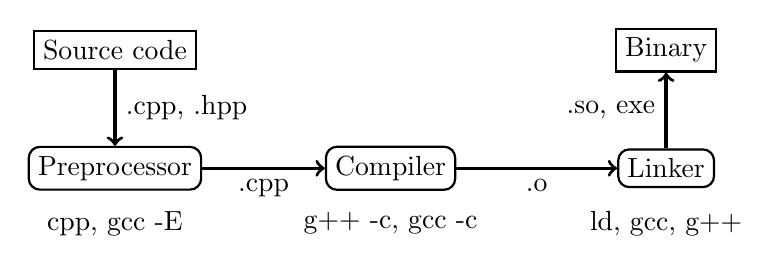
\begin{tikzpicture}
    \draw[thick] node (code) at(0,0) [rectangle,draw] {Source code}
                 node (cpp) at(0, -1.5cm) [rectangle,rounded corners,draw] {Preprocessor}
                 node (gcc) at(3.5cm,-1.5cm) [rectangle,rounded corners,draw] {Compiler}
                 node (ld) at(7cm,-1.5cm) [rectangle,rounded corners,draw] {Linker}
                 node (bin) at(7cm,0) [rectangle,draw] {Binary}
                 node at(0, -2.2cm) {cpp, gcc -E}
                 node at(3.5cm, -2.2cm) {g++ -c, gcc -c}
                 node at(7cm, -2.2cm) {ld, gcc, g++};
    \draw[very thick,->] (code) -- (cpp) node [midway,right] {.cpp, .hpp};
    \draw[very thick,->] (cpp) -- (gcc) node [midway,below] {.cpp};
    \draw[very thick,->] (gcc) -- (ld) node [midway,below] {.o};
    \draw[very thick,->] (ld) -- (bin) node [midway,left] {.so, exe};
  \end{tikzpicture}
  \begin{block}{The steps}
    \begin{description}
    \item[cpp]
        the preprocessor \\
        handles the \# directives (macros, includes) \\
        creates ``complete'' source code (ie. translation unit)
    \item[g++]
        the compiler \\
        creates machine code from \cpp code
    \item[ld]
        the linker \\
        links several binary files into libraries and executables
    \end{description}
  \end{block}
\end{frame}

\begin{frame}[fragile]
  \frametitle{Compilers}
  \begin{block}{Available tools}
    \begin{description}
    \item[\href{http://gcc.gnu.org/}{\beamergotobutton{gcc}}]
        the most common and most used\\
        free and open source
    \item[\href{http://clang.llvm.org/}{\beamergotobutton{clang}}]
        drop-in replacement of gcc \\
        slightly better error reporting \\
        free and open source, based on LLVM
    \item[\href{https://www.intel.com/content/www/us/en/developer/tools/oneapi/dpc-compiler.html\#gs.dyllp0}{\beamergotobutton{icc} \beamergotobutton{icx}}]
        Intel's compilers, proprietary but now free \\
        optimized for Intel hardware \\
        icc being replaced by icx, based on LLVM
    \item[\href{https://visualstudio.microsoft.com/}{\beamergotobutton{Visual \cpp / MSVC}}]
      Microsoft's C++ compiler on Windows
    \end{description}
  \end{block}
  \begin{alertblock}{My preferred choice today}
    \begin{itemize}
      \item \alert{gcc} as the de facto standard in HEP
      \item \hspace{0pt}\alert{clang} in parallel to catch more bugs
    \end{itemize}
  \end{alertblock}
\end{frame}

\begin{frame}[fragile]
  \frametitle{Useful compiler options (gcc/clang)}
  \begin{block}{Get more warnings}
    \begin{description}
      \item[-Wall -Wextra] get all warnings
      \item[-Werror] force yourself to look at warnings
    \end{description}
  \end{block}
  \begin{block}{Optimization}
    \begin{description}
      \item[-g] add debug symbols
      \item[-Ox] 0 = no opt., 1-2 = opt., 3 = highly opt. (maybe larger binary), g = opt. for debugging
    \end{description}
  \end{block}
  \begin{block}{Compilation environment}
    \begin{description}
      \item[\texttt{-I} \textless{}path\textgreater] where to find header files
      \item[\texttt{-L} \textless{}path\textgreater] where to find libraries
      \item[\texttt{-l} \textless{}name\textgreater] link with libname.so
      \item[\texttt{-E / -c}] stop after preprocessing / compilation
    \end{description}
  \end{block}
\end{frame}

\begin{frame}[fragile]
  \frametitle{Makefiles}
  \begin{block}{Why to use them}
    \begin{itemize}
    \item an organized way of describing building steps
    \item avoids a lot of typing
    \end{itemize}
  \end{block}
  \begin{block}{Several implementations}
    \begin{itemize}
    \item raw Makefiles: suitable for small projects
    \item cmake: portable, the current best choice
    \item automake: GNU project solution
    \end{itemize}
  \end{block}
  \begin{minted}{makefile}
    test : test.cpp libpoly.so
        $(CXX) -Wall -Wextra -o $@ $^
    libpoly.so: Polygons.cpp
        $(CXX) -Wall -Wextra -shared -fPIC -o $@ $^
    clean:
        rm -f *o *so *~ test test.sol
  \end{minted}
\end{frame}

\begin{frame}[fragile]
  \frametitle{CMake}
  \begin{block}{}
    \begin{itemize}
      \item a cross-platform meta build system
      \item generates platform-specific build systems
      \item see also this \href{https://www.youtube.com/watch?v=eC9-iRN2b04}{basic} and \href{https://www.youtube.com/watch?v=bsXLMQ6WgIk}{detailed} talks
    \end{itemize}
  \end{block}
  \begin{block}{Example CMakeLists.txt}
    \begin{minted}[linenos=true,autogobble]{cmake}
      cmake_minimum_required(VERSION 3.18)
      project(hello CXX)

      find_package(ZLIB REQUIRED) # for external libs

      add_executable(hello main.cpp util.h util.cpp)
      target_compile_features(hello PUBLIC cxx_std_17)
      target_link_libraries(hello PUBLIC ZLIB::ZLIB)
    \end{minted}
  \end{block}
\end{frame}

\begin{frame}[fragile]
  \frametitle{CMake - Building}
  \begin{block}{Building a CMake-based project}
    Start in the directory with the top-level \texttt{CMakeLists.txt}:
    \begin{minted}[linenos=true,autogobble]{bash}
      mkdir build # will contain all build-related files
      cd build
      cmake ..    # configures and generates a build system
      cmake -DCMAKE_BUILD_TYPE=Release .. # pass arguments
      ccmake .    # change configuration using terminal GUI
      cmake-gui . # change configuration using Qt GUI
      cmake --build . -j8    # build project with 8 threads
      cmake --build . --target hello  # build only hello
      sudo cmake --install . # install project into system
      cd ..
      rm -r build # clean everything
    \end{minted}
  \end{block}
\end{frame}

\begin{frame}[fragile]
  \frametitle{Compiler chain}
  \begin{alertblock}{Exercise Time}
    \begin{itemize}
    \item go to code/functions
    \item preprocess functions.cpp (cpp or gcc -E -o output)
    \item compile functions.o and Structs.o (g++ -c -o output)
    \item use nm to check symbols in .o files
    \item look at the Makefile
    \item try make clean; make
    \item see linking stage of the final program using g++ -v
      \begin{itemize}
      \item just add a -v in the Makefile command for functions target
      \item run make clean; make
      \item look at the collect 2 line, from the end up to ``-o functions''
      \end{itemize}
    \item see library dependencies with `ldd functions`
    \end{itemize}
  \end{alertblock}
\end{frame}

\subsection[gdb]{Debugging}

\begin{frame}[fragile]
  \frametitle{Debugging}
  \begin{alertblock}{The problem}
    \begin{itemize}
      \item everything compiles fine (no warning)
      \item but crashes at run time
      \item no error message, no clue
    \end{itemize}
  \end{alertblock}
  \pause
  \begin{block}{The solution : debuggers}
    \begin{itemize}
    \item dedicated program able to stop execution at any time
    \item and show you where you are and what you have
    \end{itemize}
  \end{block}
  \pause
  \begin{block}{Existing tools}
    \begin{description}
    \item[\href{http://www.sourceware.org/gdb/}{\beamergotobutton{gdb}}]
      THE main player
    \item[\href{http://lldb.llvm.org/}{\beamergotobutton{lldb}}]
      the debugger coming with clang/LLVM
    \item[\href{https://www.intel.com/content/www/us/en/develop/documentation/get-started-with-debugging-dpcpp-linux/top.html}{\beamergotobutton{gdb-oneapi}}]
      the Intel OneAPI debugger
    \end{description}
    They usually can be integrated into your IDE
  \end{block}
\end{frame}

\begin{frame}[fragile]
  \frametitle{gdb crash course}
  \begin{block}{start gdb}
    \begin{itemize}
    \item gdb \textless{}program\textgreater
    \item gdb \textless{}program\textgreater \textless{}core file\textgreater
    \item gdb -{}-args \textless{}program\textgreater \textless{}program arguments\textgreater
    \end{itemize}
  \end{block}
  \begin{block}{inspect state}
    \begin{description}
    \item[bt] prints a backtrace
    \item[print \textless{}var\textgreater] prints current content of the variable
    \item[list] show code around current point
    \item[up/down] go up or down in call stack
    \end{description}
  \end{block}
  \begin{block}{breakpoints}
    \begin{description}
    \item[break \textless{}function\textgreater] puts a breakpoint on function entry
    \item[break \textless{}file\textgreater:\textless{}line\textgreater] puts a breakpoint on that line
    \end{description}
  \end{block}
\end{frame}

\begin{frame}[fragile]
  \frametitle{gdb}
  \begin{exercise}{gdb}
    \begin{itemize}
    \item go to code/debug
    \item compile, run, see the crash
    \item run it in gdb (or lldb on newer MacOS)
    \item inspect backtrace, variables
    \item find problem and fix bug
    \item try stepping, breakpoints
    \item use -Wall -Wextra and see warning
    \end{itemize}
  \end{exercise}
\end{frame}

\subsection[sani]{Sanitizers}

\begin{frame}[fragile]
  \frametitle{Address Sanitizer (ASan)}
  \begin{block}{ASan introduction}
    \begin{itemize}
    \item Compiler instrumentation
    \item Program stops on invalid memory access, e.g.\
      \begin{itemize}
        \item Invalid read/write on heap and stack
        \item Double free/delete, use after free
        \item Buffer overflow on stack (few tools can do this)
        \item Only linux: memory leaks
      \end{itemize}
    \end{itemize}
  \end{block}
  \pause
  \begin{exampleblock}{Usage (gcc/clang syntax)}
    \begin{itemize}
    \item Compile with \mintinline{bash}{-fsanitize=address -fno-omit-frame-pointer -g}
    \item With clang, add optionally: \texttt{-fsanitize-address-use-after-return=always -fsanitize-address-use-after-scope}
    \item Link with \mintinline{bash}{-fsanitize=address}
    \item Run the program
    \end{itemize}
  \end{exampleblock}
\end{frame}

\begin{frame}[fragile]
  \frametitle{Address Sanitizer (ASan)}
  \begin{block}{How it works}
    \begin{itemize}
      \item Compiler adds run-time checks ($\sim$2x slow down)
      \item \cppinline{IsPoisoned(address)} looks up state of address in asan's ``shadow memory''
      \item Shadow memory: memory where 1 shadow byte tracks state of 8 application bytes (state = accessible, poisoned, \ldots)
      \item Functions that deal with memory (\cppinline{new() / delete()} / strings / ...) update entries in shadow memory when called
    \end{itemize}
  \end{block}
  \begin{exampleblock}{asan instrumentation (mock code)}
    \begin{overprint}
      \onslide<1>
      \vfill
      \begin{cppcode*}{}
        int i = *address;
      \end{cppcode*}
      \onslide<2->
      \vfill
      \begin{cppcode*}{}
        if (IsPoisoned(address)) {
          ReportError(address, kAccessSize, kIsWrite);
        }
        int i = *address;
      \end{cppcode*}
    \end{overprint}
  \end{exampleblock}
\end{frame}


\begin{frame}[fragile]
  \begin{block}{ASan red zones}
    \begin{itemize}
      \item If adjacent data blocks are owned by the process, the operating system will allow an access
      \item<2> ASan surrounds blocks of memory by poisoned red zones
      \item<2> Program stops when accessing a red zone
    \end{itemize}
  \end{block}
  \begin{exampleblock}{Illegal access (not detected without ASan)}
    \begin{multicols}{2}
      \begin{overprint}
        \onslide<1>
        \begin{cppcode*}{}
          void foo() {
            char a[8];
            char b[8];
            a[8] = '1';
          }
        \end{cppcode*}
        \onslide<2>
        \begin{minted}{diff}
  void foo() {
+   char redzone1[32];
    char a[8];
+   char redzone2[24];
    char b[8];
+   char redzone3[24];
+   // <poison redzones>
    a[8] = '1';
+   // <unpoison redzones>
 }
        \end{minted}
      \end{overprint}
      \columnbreak
      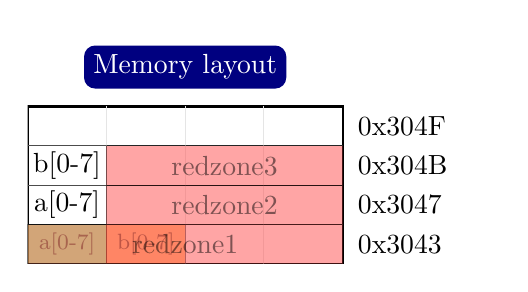
\begin{tikzpicture}
        \clip (0,0) rectangle (6cm, 3cm);
        \memorystack[word size=4,nb blocks=4]
        \onslide<1>{
          \draw[fill=green!70,opacity=0.5] (0.,0.*\stacksizey) rectangle (\stacksizex/4.,1.*\stacksizey) node[midway]{\footnotesize a[0-7]};
          \draw[fill=orange,opacity=0.5] (\stacksizex/4.,0.*\stacksizey) rectangle (\stacksizex/2.,1.*\stacksizey) node[midway]{\footnotesize b[0-7]};
        }
        \memorygoto{2}
        \onslide<2->{
          \draw[fill=red!70,opacity=0.5] (0.,0.*\stacksizey) rectangle (\stacksizex,1.*\stacksizey) node[midway]{redzone1};
          \memorypush{a[0-7]}
          \draw[fill=red!70,opacity=0.5] (0.+\stacksizex/4.,1.*\stacksizey) rectangle (\stacksizex,2.*\stacksizey) node[midway]{redzone2};
          \memorypush{b[0-7]}
          \draw[fill=red!70,opacity=0.5] (0.+\stacksizex/4.,2.*\stacksizey) rectangle (\stacksizex,3.*\stacksizey) node[midway]{redzone3};
        }
      \end{tikzpicture}
    \end{multicols}
    \vspace{1mm}
  \end{exampleblock}
\end{frame}

\begin{frame}[fragile]
  \vspace{-1\baselineskip}
  \begin{columns}
    \column{\textwidth+1cm}
    \scriptsize
    \begin{Verbatim}[commandchars=\\\{\}]
    \ttfamily
\textcolor{teal}{==34015==ERROR: AddressSanitizer: stack-buffer-overflow on address 0x7ffee93ed968 at pc 0x000106812df4 bp 0x7ffee93ed930 sp 0x7ffee93ed928}
\textcolor{blue}{WRITE of size 1 at 0x7ffee93ed968 thread T0}
    #0 0x106812df3 in foo() asan.cpp:4
    #1 0x106812ed8 in main asan.cpp:9
    #2 0x7fff6d3923d4 in start (libdyld.dylib:x86_64+0x163d4)

\textcolor{teal}{Address 0x7ffee93ed968 is located in stack of thread T0 at offset 40 in frame}
    #0 0x106812cdf in foo() asan.cpp:1

  This frame has 2 object(s):
    [32, 40) 'a' (line 2) \textcolor{teal}{<== Memory access at offset 40 overflows this variable}
    [64, 72) 'b' (line 3)
Shadow bytes around the buggy address:
=>0x1fffdd27db20: 00 00 00 00 00 00 00 00 \textcolor{red}{f1 f1 f1 f1} 00[\textcolor{red}{f2}]\textcolor{red}{f2 f2}
  0x1fffdd27db30: 00 \textcolor{red}{f3 f3 f3} 00 00 00 00 00 00 00 00 00 00 00 00
  0x1fffdd27db40: 00 00 00 00 00 00 00 00 00 00 00 00 00 00 00 00
  0x1fffdd27db50: 00 00 00 00 00 00 00 00 00 00 00 00 00 00 00 00
Shadow byte legend (one shadow byte represents 8 application bytes):
  Addressable:           00
  Partially addressable: 01 02 03 04 05 06 07
  Heap left redzone:       \textcolor{red}{fa}
  Freed heap region:       \textcolor{pink}{fd}
  Stack left redzone:      \textcolor{red}{f1}
  Stack mid redzone:       \textcolor{red}{f2}
  Stack right redzone:     \textcolor{red}{f3}
  Stack after return:      \textcolor{pink}{f5}
    \end{Verbatim}
  \end{columns}
\end{frame}

\begin{frame}[fragile]
  \begin{columns}
    \column{\textwidth+1cm}
    \begin{block}{Finding memory leaks with ASan}
      \begin{itemize}
        \item On linux, ASan can display memory leaks (``LeakSanitizer'')
        \item Might be active already, otherwise start executable with \mintinline{bash}{ASAN_OPTIONS=detect_leaks=1 ./myProgram}
      \end{itemize}
    \end{block}
    \scriptsize
    \begin{Verbatim}[commandchars=\\\{\}]
    \ttfamily
\textcolor{red}{==113262==ERROR: LeakSanitizer: detected memory leaks}

\textcolor{blue}{Direct leak of 32 byte(s) in 1 object(s) allocated from:}
  #0 0x7f2671201647 in operator new(unsigned long) /build/dkonst/WORK/build/contrib/gcc-10.1.0/src/gcc/10.1.0/libsanitizer/asan/asan_new_delete.cpp:99
  #1 0x4033c7 in memoryLeak[abi:cxx11]() /afs/cern.ch/user/s/shageboe/asan.cpp:33
  #2 0x403633 in main /afs/cern.ch/user/s/shageboe/asan.cpp:40
  #3 0x7f2670a15492 in __libc_start_main (/lib64/libc.so.6+0x23492)

\textcolor{blue}{Indirect leak of 22 byte(s) in 1 object(s) allocated from:}
  #0 0x7f2671201647 in operator new(unsigned long) /build/dkonst/WORK/build/contrib/gcc-10.1.0/src/gcc/10.1.0/libsanitizer/asan/asan_new_delete.cpp:99
  #1 0x403846 in void std::__cxx11::basic_string<char, std::char_traits<char>, std::allocator<char> >::_M_construct<char const*>(char const*, char const*, std::forward_iterator_tag) /cvmfs/sft.cern.ch/lcg/releases/gcc/10.1.0.c82-6f386/x86_64-centos8/include/c++/10.1.0/bits/basic_string.tcc:219
  #2 0x4033f4 in std::__cxx11::basic_string<char, std::char_traits<char>, std::allocator<char> >::basic_string<std::allocator<char> >(char const*, std::allocator<char> const&) /cvmfs/sft.cern.ch/lcg/releases/gcc/10.1.0.c82-6f386/x86_64-centos8/include/c++/10.1.0/bits/basic_string.h:247
  #3 0x4033f4 in memoryLeak[abi:cxx11]() /afs/cern.ch/user/s/shageboe/asan.cpp:33
  #4 0x403633 in main /afs/cern.ch/user/s/shageboe/asan.cpp:40
  #5 0x7f2670a15492 in __libc_start_main (/lib64/libc.so.6+0x23492)

SUMMARY: AddressSanitizer: 54 byte(s) leaked in 2 allocation(s).
    \end{Verbatim}
  \end{columns}
\end{frame}

\begin{frame}[fragile]
  \frametitle{Address sanitizer (ASan)}
  \begin{block}{Wrap up}
    \begin{itemize}
      \item If a program crashes, run it with asan
      \item Should be part of every \cpp{} continuous integration system
      \item It will also find bugs that by luck didn't crash the program
      \item It doesn't generate false positives
    \end{itemize}
  \end{block}

  \begin{exampleblock}{More info}
    \begin{itemize}
      \item \url{https://github.com/google/sanitizers/wiki/AddressSanitizer}
      \item Compile with asan, and start executable using \mintinline{bash}{ASAN_OPTIONS=help=1 <executable>}
    \end{itemize}
  \end{exampleblock}
\end{frame}

\begin{frame}[fragile]
  \frametitle{Address sanitizer (ASan)}
  \begin{exercise}{address sanitizer}
    \begin{itemize}
      \item Go to \texttt{exercises/asan}
      \item Compile and run the program \texttt{./asan}
      \item There are two bugs and one memory leak. Use asan to trace them down.
    \end{itemize}
  \end{exercise}

\end{frame}

\begin{frame}[fragile]
  \frametitle{Thread sanitizer (TSan)}
  \begin{block}{TSan}
    \begin{itemize}
      \item Thread sanitizer detects many data races in MT programs
      \item Recompile your program with e.g.\ \mintinline{shell}{clang++ -fsanitize=thread -g -O1 datarace.cpp}
    \end{itemize}
  \end{block}

  \footnotesize
  \begin{verbatim}
% ./a.out
WARNING: ThreadSanitizer: data race (pid=19219)
Write of size 4 at 0x7fcf47b21bc0 by thread T1:
  #0 Thread1 datarace.c:4 (exe+0x00000000a360)

Previous write of size 4 at 0x7fcf47b21bc0 by main thread:
  #0 main datarace.c:10 (exe+0x00000000a3b4)

Thread T1 (running) created at:
  #0 pthread_create tsan_interceptors.cc:705 (exe+0x00000000c790)
  #1 main datarace.c:9 (exe+0x00000000a3a4)
  \end{verbatim}

  \begin{block}{}
    \scriptsize
    \url{https://github.com/google/sanitizers/wiki/ThreadSanitizerCppManual}
  \end{block}
\end{frame}

\begin{frame}[fragile]
  \frametitle{Undefined Behaviour Sanitizer (UBSan)}
  \begin{block}{UBSan}
    \begin{itemize}
      \item Tracks uninitialised memory, broken arithmetic, wrong array indexing and other undefined behaviour
      \item Recompile your program with e.g.\ \mintinline{bash}{clang++ -fsanitize=undefined -g -O1 ub.cpp}
    \end{itemize}
  \end{block}
  \small
  \begin{verbatim}
% ./a.out
up.cpp:3:5: runtime error: signed integer overflow:
            2147483647 + 1 cannot be represented in type 'int'
  \end{verbatim}
  \begin{block}{}
    \footnotesize
    \url{https://clang.llvm.org/docs/UndefinedBehaviorSanitizer.html}
  \end{block}
\end{frame}

\begin{frame}[fragile]
  \frametitle{Undefined Behaviour Sanitizer (UBSan)}
  \begin{exercise}{Finding evil run-time bugs}
    \begin{itemize}
      \item Go to \texttt{exercises/ubsan}
      \item Compile and run the program following the instructions in README or in the program
      \item The program should run without observable issues
      \item Recompile with UBSan and see that almost every second line contains evil bugs
    \end{itemize}
  \end{exercise}

\end{frame}

\subsection[valgrind]{The Valgrind family}

\begin{frame}[fragile]
  \frametitle{The valgrind family}
  \begin{block}{Valgrind fundamentals}
    \begin{itemize}
    \item valgrind is a framework for different tools
    \item a processor simulator allowing checks in between instructions
    \item slow (10-50 times slower than normal execution)
    \item easy to use : ``valgrind \textless{}your executable\textgreater''
      \begin{itemize}
      \item no recompilation
      \item better with -g -O0, but not strictly needed
      \end{itemize}
    \item it is free and open source
    \end{itemize}
  \end{block}
  \pause
  \begin{block}{Main tools}
    \begin{description}
      \item[memcheck] a memory checker (default tool) and leak detector
      \item[callgrind] a call graph builder
      \item[helgrind] a race condition detector
    \end{description}
  \end{block}
\end{frame}

\begin{frame}[fragile]
  \frametitle{memcheck}
  \begin{block}{}
    \begin{itemize}
      \item keeps track of all memory allocations and deallocations
      \item is able to detect accesses to unallocated memory
      \item and even tell you when it was deallocated if it was
      \item or what is the closest array in case of overflow
      \item is able to list still allocated memory when program exits\\
        (memory leaks detection)
    \end{itemize}
  \end{block}
\end{frame}

\begin{frame}[fragile]
  \frametitle{valgrind}
  \begin{alertblock}{Exercise Time}
    \begin{itemize}
    \item go to code/valgrind
    \item compile, run, it should work
    \item run with valgrind, see the problem
    \item fix the problem
      \vspace{.3cm}
    \item go back to the code/debug exercise
    \item check it with valgrind
    \item analyze the issue, see that the variance was biaised
    \item fix the issue
    \end{itemize}
  \end{alertblock}
\end{frame}

\begin{frame}[fragile]
  \frametitle{memcheck}
  \begin{alertblock}{Exercise Time}
    \begin{itemize}
    \item go to code/memcheck
    \item compile, run, it should work
    \item run with valgrind, see LEAK summary
    \item run with -{}-leak-check=full to get details
    \item analyze and correct it
    \end{itemize}
  \end{alertblock}
\end{frame}

\begin{frame}[fragile]
  \frametitle{callgrind and kcachegrind}
  \begin{block}{callgrind}
    \begin{itemize}
      \item keeps track of all function calls
      \item and time spent in each function
      \item build statistics on calls, CPU usages and more
      \item outputs flat statistics file, quite unreadable
    \end{itemize}
  \end{block}
  \begin{block}{kcachegrind}
    \begin{itemize}
      \item a gui exploiting statistics built by callgrind
      \item able to browse graphically the program calls
      \item able to ``graph'' CPU usage on the program structure
    \end{itemize}
  \end{block}
\end{frame}

\begin{frame}[fragile]
  \frametitle{callgrind}
  \begin{alertblock}{Exercise Time}
    \begin{itemize}
    \item go to code/callgrind
    \item compile, run, it will be slow
    \item change nb iterations to 20
    \item run with valgrind -{}-tool=callgrind
    \item look at output with kcachegrind
    \item change fibo call to fibo2
    \item observe the change in kcachegrind
    \end{itemize}
  \end{alertblock}
\end{frame}

\begin{frame}[fragile]
  \frametitle{helgrind}
  \begin{block}{}
    \begin{itemize}
      \item keeps track of all pthreads activity
      \item in particular keeps track of all mutexes
      \item builds a graph of dependencies of the different actions
      \item works on the resulting graph to detect:
        \begin{itemize}
        \item possible dead locks
        \item possible data races
        \end{itemize}
    \end{itemize}
  \end{block}
  \pause
  \begin{alertblock}{}
    Note the ``possible''. It finds future problems !
  \end{alertblock}
\end{frame}

\begin{frame}[fragile]
  \frametitle{helgrind}
  \begin{alertblock}{Exercise Time}
    \begin{itemize}
    \item go to code/helgrind
    \item compile, run
    \item check it with valgrind. You may see strange behavior \\
      or it will be perfectly fine
    \item check it with valgrind -{}-tool=helgrind
    \item understand issue and fix
    \end{itemize}
  \end{alertblock}
\end{frame}

\subsection[static]{Static code analysis}

\begin{frame}[fragile]
  \frametitle{Static analysis}
  \begin{alertblock}{The problem}
    \begin{itemize}
    \item all the tools discussed so far work on binaries
    \item they analyze the code being run
    \item so there is a coverage problem (e.g. for error cases)
    \end{itemize}
  \end{alertblock}
  \pause
  \begin{block}{A (partial) solution : analyzing the source code}
    \begin{itemize}
    \item build a graph of dependencies of the calls
    \item use graph tools to detect potential memory corruptions,
      memory leaks or missing initializations
    \end{itemize}
  \end{block}
  \pause
  \begin{block}{Existing tools}
    \begin{description}
    \item[\href{http://www.coverity.com/}{\beamergotobutton{Coverity}}]
      proprietary tool, the most complete
    \item[\href{http://cppcheck.sourceforge.net/}{\beamergotobutton{cppcheck}}]
      free and opensource, but less complete
    \item[\href{https://clang.llvm.org/extra/clang-tidy/}{\beamergotobutton{clang-tidy}}]
      clang-based ``linter'', includes clang static analyzer
    \end{description}
  \end{block}
\end{frame}

\begin{frame}[fragile]
  \frametitle{cppcheck}
  \begin{exercise}{cppcheck}
    \begin{itemize}
    \item go to \texttt{exercises/cppcheck}
    \item compile, run, see that it works
    \item use valgrind: no issue
    \item use cppcheck, see the problem
    \item analyze the issue, and fix it
    \item bonus: understand why valgrind did not complain \\
      and how the standard deviation could be biased \\
      hint : use gdb and check addresses of v and diffs
    \end{itemize}
  \end{exercise}
\end{frame}

\begin{frame}[fragile]
  \frametitle{clang-tidy}
  \begin{block}{Documentation and supported checks}
    \begin{itemize}
      \item \url{https://clang.llvm.org/extra/clang-tidy/}
    \end{itemize}
  \end{block}
  \begin{block}{Run clang-tidy}
    \begin{itemize}
      \item \mintinline{bash}{clang-tidy <file.cpp> -checks=...}
      \item \mintinline{bash}{clang-tidy <file.cpp>} (checks from .clang-tidy file)
      \item \mintinline{bash}{clang-tidy <file.cpp> --fix} (applies fixes)

    \end{itemize}
  \end{block}
  \begin{block}{Compilation flags}
    \begin{itemize}
      \item clang-tidy needs to know exactly how your program is built
      \item \mintinline{bash}{clang-tidy ... -- <all compiler flags>}
    \end{itemize}
  \end{block}
  \begin{block}{.clang-tidy file}
    \begin{itemize}
      \item describes which checks to run
      \item usually checked in at repository root
    \end{itemize}
  \end{block}
\end{frame}

\begin{frame}[fragile]
  \begin{block}{Automatically collecting compilation flags}
    \begin{itemize}
      \item clang-tidy looks for a file called compile\_commands.json
      \item contains the exact build flags for each .cpp file
      \item generate with CMake: \\
        \mintinline{bash}{cmake -DCMAKE_EXPORT_COMPILE_COMMANDS=ON ...}
      \item for Makefiles try \href{https://github.com/rizsotto/Bear}{\beamergotobutton{Bear}}
      \item allows to run clang-tidy in bulk on all files:
      \begin{itemize}
        \item \mintinline{bash}{run-clang-tidy -checks ...}
        \item \mintinline{bash}{run-clang-tidy} (checks from .clang-tidy)
        \item \mintinline{bash}{run-clang-tidy -fix} (applies fixes)
      \end{itemize}
    \end{itemize}
  \end{block}
\end{frame}

\begin{frame}[fragile]
  \frametitle{clang-tidy}
  \begin{exercise}{clang-tidy}
    \begin{itemize}
      \item go to any example which compiles (e.g. \texttt{exercises/cppcheck})
      \item \mintinline{bash}{mkdir build && cd build}
      \item \mintinline{bash}{cmake -DCMAKE_EXPORT_COMPILE_COMMANDS=ON ..}
      \item \mintinline{bash}{clang-tidy <../file.cpp> -checks=*}
      \item inspect output
      \item run with \mintinline{bash}{--fix} flag
      \item revert changes using \mintinline{bash}{git checkout <../file.cpp>}
    \end{itemize}
  \end{exercise}
\end{frame}


\section[conc]{Concurrency}

\subsection[thr]{Threads and async}

\begin{frame}[fragile]
  \frametitlecpp[11]{Basic concurrency}
  \begin{block}{Threading}
    \begin{itemize}
    \item new object std::thread in \textless{}thread\textgreater{} header
    \item takes a function as argument of its constructor
    \item must be detached or joined before the main thread terminates
    \item \cpp20: std::jthread automatically joins at destruction
    \end{itemize}
  \end{block}
  \pause
  \begin{exampleblock}{Example code}
    \begin{cppcode*}{}
      void doSth() {...}
      void doSthElse() {...}
      int main() {
        std::thread t1(doSth);
        std::thread t2(doSthElse);
        for (auto t: {&t1,&t2}) t->join();
      }
    \end{cppcode*}
  \end{exampleblock}
\end{frame}

\begin{frame}[fragile]
  \frametitlecpp[11]{The thread constructor}
  \begin{exampleblock}{Can take a function and its arguments}
    \begin{cppcode*}{}
      void function(int j, double j) {...};
      std::thread t1(function, 1, 2.0);
    \end{cppcode*}
  \end{exampleblock}
  \pause
  \begin{exampleblock}{Can take any function-like object}
    \begin{cppcode*}{}
      struct AdderFunctor {
        AdderFunctor(int i): m_i(i) {}
        int operator() (int j) const { return i+j; };
        int m_i;
      };
      std::thread t2(AdderFunctor(2), 5);
      int a;
      std::thread t3([](int i) { return i+2; }, a);
      std::thread t4([a]       { return a+2; });
    \end{cppcode*}
  \end{exampleblock}
\end{frame}

\begin{frame}[fragile]
  \frametitlecpp[11]{Basic asynchronicity}
  \begin{block}{Concept}
    \begin{itemize}
    \item separation of the specification of what should be done and the retrieval of the results
    \item ``start working on this, and ping me when it's ready''
    \end{itemize}
  \end{block}
  \pause
  \begin{block}{Practically}
    \begin{itemize}
    \item std::async function launches an asynchronous task
    \item std::future template allows to handle the result
    \end{itemize}
  \end{block}
  \pause
  \begin{exampleblock}{Example code}
    \begin{cppcode*}{}
      int computeSth() {...}
      std::future<int> res = std::async(computeSth);
      std::cout << res->get() << std::endl;
    \end{cppcode*}
  \end{exampleblock}
\end{frame}

\begin{frame}[fragile]
  \frametitlecpp[11]{Mixing the two}
  \begin{block}{Is async running concurrent code ?}
    \begin{itemize}
    \item it depends !
    \item you can control this with a launch policy argument
      \begin{description}
      \item[std::launch::async] spawns a thread for immediate execution
      \item[std::launch::deferred] causes lazy execution in current thread
      \end{description}
      \begin{itemize}
      \item execution starts when get() is called
      \end{itemize}
    \item default is not specified !
    \end{itemize}
  \end{block}
  \pause
  \begin{exampleblock}{Usage}
    \begin{cppcode*}{}
      int computeSth() {...}
      auto res = std::async(std::launch::async,
                            computeSth);
      auto res2 = std::async(std::launch::deferred,
                             computeSth);
    \end{cppcode*}
  \end{exampleblock}
\end{frame}

\begin{frame}[fragile]
  \frametitlecpp[11]{Fine grained control on asynchronous execution}
  \begin{block}{std::packaged\_task template}
    \begin{itemize}
    \item creates an asynchronous version of any function-like object
      \begin{itemize}
      \item identical arguments
      \item returns a std::future
      \end{itemize}
    \item provides access to the returned future
    \item associated with threads, gives full control on execution
    \end{itemize}
  \end{block}
  \pause
  \begin{exampleblock}{Usage}
    \begin{cppcode*}{}
      int task() { return 42; }
      std::packaged_task<int()> pckd_task(task);
      auto future = pckd_task.get_future();
      pckd_task();
      std::cout << future.get() << std::endl;
    \end{cppcode*}
  \end{exampleblock}
\end{frame}

\subsection[mutex]{Mutexes}

\begin{frame}[fragile]
  \frametitlecpp[11]{Races}
  \begin{exampleblockGB}{Example code}{https://godbolt.org/z/oGz61Pn19}{Race}
    \begin{cppcode*}{}
      int a = 0;
      void inc() { a++; };
      void inc100() {
        for (int i=0; i < 100; i++) inc();
      };
      int main() {
        std::thread t1{inc100};
        std::thread t2{inc100};
        for (auto t: {&t1,&t2}) t->join();
        std::cout << a << "\n";
      }
    \end{cppcode*}
  \end{exampleblockGB}
  \pause
  \begin{block}{What do you expect? (Exercise exercises/race)}
    \pause
    Anything between 100 and 200 !!!
  \end{block}
\end{frame}

\begin{frame}[fragile]
  \frametitlecpp[11]{Atomicity}
  \begin{exampleblock}{Definition (wikipedia)}
    \begin{itemize}
    \item an operation (or set of operations) is atomic if it appears to the rest of the system to occur instantaneously
    \end{itemize}
  \end{exampleblock}
  \begin{block}{Practically}
    \begin{itemize}
    \item an operation that won't be interrupted by other concurrent operations
    \item an operation that will have a stable environment during execution
    \end{itemize}
  \end{block}
  \pause
  \begin{alertblock}{Is \texttt{++} operator atomic ?}
    \pause
    Usually not. It behaves like :
    \begin{cppcode*}{}
      eax = a       // memory to register copy
      increase eax  // increase (atomic CPU instruction)
      a = eax       // copy back to memory
    \end{cppcode*}
  \end{alertblock}
\end{frame}

\begin{frame}[fragile]
  \frametitlecpp[11]{Timing}
  \begin{exampleblock}{Code}
    \begin{cppcode*}{}
      eax = a       // memory to register copy
      increase eax  // increase (atomic CPU instruction)
      a = eax       // copy back to memory
    \end{cppcode*}
  \end{exampleblock}
  \begin{block}{For 2 threads}
    \begin{tikzpicture}
      \begin{umlseqdiag}
        \umlobject[x=0, class=eax]{Thread 1}
        \umlobject[x=3, class=a, fill=blue!20]{Memory}
        \umlobject[x=6, class=eax]{Thread 2}
        \begin{umlcall}[op=read, type=synchron, return=0]{Thread 1}{Memory}
        \end{umlcall}
        \begin{umlcall}[padding=3, op=read, type=synchron, return=0]{Thread 2}{Memory}
        \end{umlcall}
        \begin{umlcallself}[op=incr, type=synchron]{Thread 1}
        \end{umlcallself}
        \begin{umlcallself}[op=incr, type=synchron]{Thread 2}
        \end{umlcallself}
        \begin{umlcall}[op=write 1]{Thread 2}{Memory}
        \end{umlcall}
        \begin{umlcall}[padding=3, op=write 1]{Thread 1}{Memory}
        \end{umlcall}
      \end{umlseqdiag}
      \draw[-triangle 60](8.5,0) -- (8.5,-4) node[right, pos=0.5]{time};
    \end{tikzpicture}
  \end{block}
\end{frame}

\begin{frame}[fragile]
  \frametitlecpp[17]{Mutexes and Locks}
  \begin{block}{Concept}
    \begin{itemize}
    \item Use locks to serialize access to a non-atomic piece of code
    \end{itemize}
  \end{block}
  \pause
  \begin{block}{The objects}
    \begin{description}[labelwidth=1.8cm]
    \item[std::mutex] in the \cppinline{mutex} header. \textbf{Mut}ual \textbf{ex}clusion
    \item[std::scoped\_lock] RAII to lock and unlock automatically
    \item[std::unique\_lock] same, but can be released/relocked explicitly
    \end{description}
  \end{block}
  \pause
  \begin{exampleblockGB}{Practically}{https://godbolt.org/z/a5TaaPrad}{\texttt{mutex}}
    \begin{cppcode*}{}
      int a = 0;
      std::mutex m;
      void inc() {
        std::scoped_lock lock{m};
        a++;
      }
    \end{cppcode*}
  \end{exampleblockGB}
\end{frame}

\begin{frame}[fragile]
  \frametitlecpp[17]{Mutexes and Locks}
  \begin{goodpractice}{Locking}
    \begin{itemize}
      \item Generally, use \cppinline{std::scoped_lock}. Before \cpp17 use \cppinline{std::lock_guard}.
      \item Hold as short as possible, consider wrapping critical section in block statement \cppinline|{ }|
      \item Only if manual control needed, use \cppinline{std::unique_lock}
    \end{itemize}
  \end{goodpractice}
  \begin{exampleblock}{}
    \begin{cppcode*}{gobble=2}
      void function(...) {
        // uncritical work ...
        {
          std::scoped_lock myLocks{mutex1, mutex2, ...};
          // critical section
        }
        // uncritical work ...
      }
    \end{cppcode*}
  \end{exampleblock}
\end{frame}

\begin{frame}[fragile]
  \frametitle{Mutexes and Locks}
  \begin{exerciseWithShortcut}{Mutexes and Locks}{Mutexes/Locks}
    \begin{itemize}
    \item Go to \texttt{exercises/race}
    \item Look at the code and try it\\
      See that it has a race condition
    \item Use a mutex to fix the issue
    \item See the difference in execution time
    \end{itemize}
  \end{exerciseWithShortcut}
\end{frame}

\begin{frame}[fragile]
  \frametitlecpp[11]{Dead locks}
  \begin{block}{Scenario}
    \begin{itemize}
    \item 2 mutexes, 2 threads
    \item locking order different in the 2 threads
    \end{itemize}
  \end{block}
  \pause
  \begin{block}{Sequence diagram}
    \begin{tikzpicture}
      \begin{umlseqdiag}
        \umlobject[x=0]{Thread 1}
        \umlobject[x=2.5, fill=blue!20]{Mutex A}
        \umlobject[x=5, fill=blue!20]{Mutex B}
        \umlobject[x=7.5]{Thread 2}
        \begin{umlcall}[op=lock]{Thread 1}{Mutex A}
        \end{umlcall}
        \begin{umlcall}[op=lock, dt=6]{Thread 2}{Mutex B}
        \end{umlcall}
        \begin{umlcall}[op=lock (block), dt=6]{Thread 1}{Mutex B}
        \end{umlcall}
        \begin{umlcall}[op=lock (block), dt=12]{Thread 2}{Mutex A}
        \end{umlcall}
      \end{umlseqdiag}
      \draw[-triangle 60](9,0) -- (9,-4) node[right, pos=0.5]{time};
    \end{tikzpicture}
  \end{block}
\end{frame}

\begin{frame}[fragile]
  \frametitlecpp[11]{How to avoid dead locks}
  \begin{block}{Possible solutions}
    \begin{itemize}
    \item \cpp17: \cppinline{std::scoped_lock lock{m1, m2};} comes with deadlock-avoidance algorithm
    \item Never take several locks
      \begin{itemize}
      \item Or add master lock protecting the locking phase
      \end{itemize}
    \item Respect a strict locking order across all threads
    \item Do not use locks
      \begin{itemize}
      \item Use other techniques, e.g.\ lock-free queues
      \end{itemize}
    \end{itemize}
  \end{block}
\end{frame}

\begin{frame}[fragile]
  \frametitlecpp[17]{Shared mutex / locks}
  \begin{block}{Sharing a mutex}
    \begin{itemize}
      \item Normal \cppinline{std::mutex} objects cannot be shared
      \item \cppinline{std::shared_mutex} to the rescue, but can be slower
      \item It locks \emph{either} in exclusive \emph{or} in shared mode; never both
    \end{itemize}
  \end{block}
  \begin{exampleblock}{}
    \begin{cppcode*}{gobble=2}
      Data data; std::shared_mutex mutex;
      auto reader = [&](){
        std::shared_lock lock{mutex};
        read(data); // Many can read
      };
      std::thread r1{reader}, r2{reader}, ...;

      std::thread writer([&](){
        std::scoped_lock lock{mutex}; // exclusive
        modify(data); // Only one can write
      });
    \end{cppcode*}
  \end{exampleblock}
\end{frame}

\subsection[atomic]{Atomic types}

\begin{frame}[fragile]
  \frametitlecpp[11]{Atomic types in \cpp}
  \begin{block}{\texttt{std::atomic} template}
    \begin{itemize}
      \item Any trivially copyable type can be made atomic in C++
      \item Most useful for integral types
      \item May internally use locks for custom types
    \end{itemize}
  \end{block}
  \begin{exampleblock}{}
    \begin{cppcode*}{}
      std::atomic<int> a{0};
      std::thread t1([&](){ a++; });
      std::thread t2([&](){ a++; });
      a += 2;
      t1.join(); t2.join();
      assert( a == 4 ); // Guaranteed to succeed
    \end{cppcode*}
  \end{exampleblock}
\end{frame}

\begin{frame}[fragile]
  \begin{alertblock}{Expressions using an atomic type are \textit{not} atomic!}
    \begin{itemize}
      \item Atomic load; value+2; atomic store
    \end{itemize}
    \begin{cppcode*}{}
      std::atomic<int> a{0};
      std::thread t1([&]{ a = a + 2; });
      std::thread t2([&]{ a = a + 2; });
    \end{cppcode*}
  \end{alertblock}
  \begin{block}{Sequence diagram}
    \begin{tikzpicture}
      \begin{umlseqdiag}
        \umlobject[x=0]{Thread 1}
        \umlobject[x=3, fill=blue!20]{atomic}
        \umlobject[x=6]{Thread 2}
        \begin{umlcall}[op=load]{Thread 1}{atomic}
        \end{umlcall}
        \begin{umlcall}[op=+2]{Thread 1}{Thread 1}
        \end{umlcall}
        \begin{umlcall}[op=load]{Thread 2}{atomic}
        \end{umlcall}
        \begin{umlcall}[op=+2]{Thread 2}{Thread 2}
        \end{umlcall}
        \begin{umlcall}[op=store 2]{Thread 1}{atomic}
        \end{umlcall}
        \begin{umlcall}[op=store 2]{Thread 2}{atomic}
        \end{umlcall}
      \end{umlseqdiag}
      \draw[-triangle 60](9,0) -- (9,-4) node[right, pos=0.5]{time};
    \end{tikzpicture}
  \end{block}
\end{frame}

\begin{frame}[fragile]
  \begin{block}{Use atomic member functions}
    \begin{itemize}
      \item The member functions of \mintinline{cpp}{std::atomic} are thread safe
      \item \mintinline{cpp}{fetch_add} and \mintinline{cpp}{operator+=}: atomic \{ load; add; store \}
      \item But don't confuse ``\mintinline{cpp}{a += 2}'' and ``\mintinline{cpp}{a = a + 2}''
    \end{itemize}
  \end{block}
  \begin{exampleblock}{}
    \begin{cppcode*}{}
      std::atomic<int> a{0};
      std::thread t1([&]{ a.fetch_add(2); });
      std::thread t2([&]{ a += 2; });
    \end{cppcode*}
  \end{exampleblock}
  \begin{block}{Sequence diagram}
    \begin{tikzpicture}
      \begin{umlseqdiag}
        \umlobject[x=0]{Thread 1}
        \umlobject[x=3, fill=blue!20]{atomic}
        \umlobject[x=6]{Thread 2}
        \begin{umlcall}[op=fetch\_add]{Thread 1}{atomic}
        \end{umlcall}
        \begin{umlcall}[op=\texttt{+=}, dt=9]{Thread 2}{atomic}
        \end{umlcall}
      \end{umlseqdiag}
      \draw[-triangle 60](9,0) -- (9,-2) node[right, pos=0.5]{time};
    \end{tikzpicture}
  \end{block}
\end{frame}

\begin{frame}[fragile]
  \frametitlecpp[20]{Atomic references}
  \begin{block}{\texttt{std::atomic\_ref} template}
    \begin{itemize}
      \item Wraps a \mintinline{cpp}{T&} and makes access to it atomic
      \item Like \mintinline{cpp}{std::atomic<T>}, but does not contain the \mintinline{cpp}{T}
    \end{itemize}
  \end{block}
  \begin{exampleblock}{}
    \begin{cppcode*}{gobble=2}
      int a{0};
      std::thread t1([&]{ std::atomic_ref<int> r{a}; r++;});
      std::thread t2([&]{ std::atomic_ref{a}++; });
      t1.join(); t2.join();
      a += 2; // non-atomic (fine, threads joined before)
      assert( a == 4 ); // Guaranteed to succeed
    \end{cppcode*}
  \end{exampleblock}
  \begin{alertblock}{Don't mix concurrent atomic and non-atomic access}
    \begin{cppcode*}{gobble=2}
      std::thread t3([&]{ std::atomic_ref{a}++; });
      a += 2; // data race
      t3.join();
    \end{cppcode*}
  \end{alertblock}
\end{frame}

\begin{frame}[fragile]
  \frametitle{Atomic types in \cpp}
  \begin{exercise}{Atomics}
    \begin{itemize}
      \item Go to \texttt{code/atomic}
      \item You'll find a program with the same race condition as in \texttt{race}
      \item Fix it using \mintinline{cpp}{std::atomic}
    \end{itemize}
  \end{exercise}
\end{frame}

\subsection[condition]{Condition Variables}

\begin{frame}[fragile]
  \frametitlecpp[11]{Condition variables}
  \begin{block}{Communicating thread dependencies}
    \begin{itemize}
      \item \mintinline{cpp}{std::condition_variable} from \mintinline{cpp}{<condition_variable>} header
      \item Allows for a thread to sleep (= conserve CPU time) until a given condition is satisfied
    \end{itemize}
  \end{block}
  \pause
  \begin{block}{Usage}
    \begin{itemize}
    \item Use RAII-style locks to protect shared data
    \item \mintinline{cpp}{wait()} will block until the condition is met
      \begin{itemize}
      \item you can have several waiters sharing the same mutex
      \end{itemize}
    \item \mintinline{cpp}{notify_one()} will wake up one waiter
    \item \mintinline{cpp}{notify_all()} will wake up all waiters
    \end{itemize}
  \end{block}
\end{frame}

\begin{frame}[fragile]
  \frametitlecpp[17]{Using condition variables}
  \begin{block}{Producer side}
    \begin{itemize}
      \item Imagine multiple threads sharing data. Protect it with a mutex
      \item Use a condition variable to notify consumers
      \item Optimization: Don't hold lock while notifying (would block the waking threads)
    \end{itemize}
  \end{block}
  \begin{exampleblock}{}
    \begin{cppcode*}{}
      std::mutex mutex;
      std::condition_variable cond;
      Data data;
      std::thread producer([&](){
        {
          std::scoped_lock lock{mutex};
          data = produceData(); // may take long ...
        }
        cond.notify_all();
      });
    \end{cppcode*}
  \end{exampleblock}
\end{frame}

\begin{frame}[fragile]
  \begin{overprint}
  \onslide<1>
  \begin{block}{Consumer side I: Going into wait}
    \begin{itemize}
      \item Start many threads which have to wait for shared data
      \item Provide a lock to be managed by \mintinline{cpp}{wait}
      \item \mintinline{cpp}{wait} will only lock while necessary; unlocked while sleeping
      \item Threads might wake up, but \mintinline{cpp}{wait} returns only when condition satisfied
    \end{itemize}
  \end{block}
  \onslide<2->
  \begin{block}{Consumer side II: Waking up}
    \begin{itemize}
      \item \mintinline{cpp}{notify_all()} is called, threads wake up
      \item Threads try to acquire mutex, evaluate condition
      \item One thread succeeds to acquire mutex, exits from \mintinline{cpp}{wait}
      \item \alt<2>{ {\color{red} Problem}: Other threads still blocked!}{ {\color{green!80!black} Solution:} Put locking and waiting in a scope}
    \end{itemize}
  \end{block}
  \end{overprint}

  \begin{exampleblock}{}
    \begin{overprint}
    \onslide<1-2>
    \begin{cppcode*}{gobble=2,highlightlines=4}
      auto processData = [&](){

        std::unique_lock<std::mutex> lock{mutex};
        cond.wait(lock, [&](){ return data.isReady(); });

        process(data);
      };
      std::thread t1{processData}, t2{processData}, ...;
      for (auto t : {&producer, &t1, &t2, ...}) t->join();
    \end{cppcode*}

    \onslide<3>
    \begin{cppcode*}{gobble=2}
      auto processData = [&](){
        {
          std::unique_lock<std::mutex> lock{mutex};
          cond.wait(lock, [&](){ return data.isReady(); });
        }
        process(data);
      };
      std::thread t1{processData}, t2{processData}, ...;
      for (auto t : {&producer, &t1, &t2, ...}) t->join();
    \end{cppcode*}
    \end{overprint}
  \end{exampleblock}
\end{frame}

\begin{frame}[fragile]
  \frametitle{Condition variables}
  \begin{exerciseWithShortcut}{Condition variables}{Condition vars}
    \begin{itemize}
    \item Go to code/condition\_variable
    \item Look at the code and run it\\
      See that it has a race condition
    \item Fix the race condition in the usage of the condition variable
    \item Try to make threads process data in parallel
    \end{itemize}
  \end{exerciseWithShortcut}
\end{frame}


\section[py]{\cpp and python}

\subsection[module]{Writing a module}

\begin{frame}[fragile]
  \frametitle{How to build a python 3 module around \cpp code}
  \begin{block}{\cpp code : mandel.hpp}
    \begin{cppcode*}{}
      int mandel(Complex const & a);
    \end{cppcode*}
  \end{block}
\end{frame}

\begin{frame}[fragile]
  \frametitle{Basic Module(1) : wrap your method}
  \begin{block}{mandelModule.cpp - see code/python exercise}
    \begin{cppcode*}{}
      #include <Python.h>
      #include "mandel.hpp"
      PyObject * mandel_wrapper(PyObject * self,
                                PyObject * args) {
        // Parse Input
        float r, i;
        if (!PyArg_ParseTuple(args, "ff", &r, &i))
          return NULL;
        // Call C++ function
        int result = mandel(Complex(r, i));
        // Build returned objects
        return PyLong_FromLong(result);
      }
    \end{cppcode*}
  \end{block}
\end{frame}

\begin{frame}[fragile]
  \frametitle{Basic Module(2) : create the python module}
  \begin{block}{mandelModule.cpp - see code/python exercise}
    \begin{cppcode*}{}
      // declare the modules' methods
      PyMethodDef mandelMethods[] = {
          {"mandel", mandel_wrapper, METH_VARARGS,
          "computes nb of iterations for mandelbrot set"},
          {NULL, NULL, 0, NULL}
      };
      // declare the module
      struct PyModuleDef mandelModule = {
        PyModuleDef_HEAD_INIT,
        "mandel", NULL, -1, mandelMethods
      };
      PyMODINIT_FUNC PyInit_mandel(void) {
        return PyModule_Create(&mandelModule);
      }
    \end{cppcode*}
  \end{block}
\end{frame}

\begin{frame}[fragile]
  \frametitle{Basic Module(3) : use it}
  \begin{block}{First compile the module}
    \begin{itemize}
    \item as a regular shared library
    \item with '-I \$(PYTHON\_INCLUDE)'
    \end{itemize}
  \end{block}
  \begin{block}{mandel.py - see code/python exercise}
    \begin{minted}[gobble=4]{python}
      from mandel import mandel
      v = mandel(0.7, 1.2)
    \end{minted}
  \end{block}
\end{frame}


\subsection[C]{Marrying \cpp and C}

\begin{frame}[fragile]
  \frametitle{A question of mangling}
  \begin{block}{Mangling}
    the act of converting the name of variable or function to a symbol name in the binary code
  \end{block}
  \begin{block}{C versus \cpp symbol names}
    \begin{itemize}
    \item C uses bare function name
    \item \cpp allows overloading of functions by taking the signature into account
    \item so \cpp mangling has to contain signature
    \end{itemize}
  \end{block}
\end{frame}

\begin{frame}[fragile]
  \frametitle{C mangling}
  \begin{exampleblock}{Source : file.c}
    \begin{cppcode*}{}
      float sum(float a, float b);
      int square(int a);
      // won't compile : conflicting types for ‘square’
      // float square(float a);
    \end{cppcode*}
  \end{exampleblock}
  \begin{block}{Binary symbols : file.o}
    \begin{minted}[gobble=4]{shell}
      # nm file.o
      000000000000001a T square
      0000000000000000 T sum
    \end{minted}
  \end{block}
\end{frame}

\begin{frame}[fragile]
  \frametitle{\cpp mangling}
  \begin{exampleblock}{Source : file.cpp}
    \begin{cppcode*}{}
      float sum(float a, float b);
      int square(int a);
      // ok, signature is different
      float square(float a);
    \end{cppcode*}
  \end{exampleblock}
  \begin{block}{Binary symbols : file.o}
    \begin{minted}[gobble=4]{shell}
      # nm file.o
      0000000000000000 T _Z3sumff
      000000000000002a T _Z6squaref
      000000000000001a T _Z6squarei
    \end{minted}
  \end{block}
\end{frame}

\begin{frame}[fragile]
  \frametitle{Forcing C mangling in \cpp}
  \begin{block}{extern ``C''}
    These functions will use C mangling :
    \begin{cppcode*}{gobble=1}
      extern "C" {
        float sum(float a, float b);
        int square(int a);
      }
    \end{cppcode*}
  \end{block}
  \pause
  You can now call these \cpp functions from C code
  \pause
  \begin{alertblock}{Limitations}
    \begin{itemize}
    \item no \cpp types should go out
    \item no exceptions either (use noexcept here)
    \item member functions cannot be used
      \begin{itemize}
      \item they need to be wrapped one by one
      \end{itemize}
    \end{itemize}
  \end{alertblock}
\end{frame}

\subsection[ctypes]{The ctypes module}

\begin{frame}[fragile]
  \frametitle{The ctypes python module}
  \begin{block}{From the documentation}
    \begin{itemize}
    \item provides C compatible data types
    \item allows calling functions in DLLs or shared libraries
    \item can be used to wrap these libraries in pure Python
    \end{itemize}
  \end{block}
\end{frame}

\begin{frame}[fragile]
  \frametitle{ctypes : usage example}
  \begin{block}{\cpp code : mandel.hpp}
    \begin{cppcode*}{}
      int mandel(Complex const & a);
    \end{cppcode*}
  \end{block}
  \begin{block}{``C'' code : mandel\_cwrapper.hpp}
    \begin{cppcode*}{}
      extern "C" {
        int mandel(float r, float i) {
          return mandel(Complex(r, i));
        };
      }
    \end{cppcode*}
  \end{block}
  \begin{exampleblock}{calling the mandel library}
    \begin{minted}[gobble=4]{python}
      from ctypes import *
      libmandel = CDLL('libmandelc.so')
      v = libmandel.mandel(c_float(0.3), c_float(1.2))
    \end{minted}
  \end{exampleblock}
\end{frame}

\begin{frame}
  \frametitle{Marrying \cpp and python}
  \begin{alertblock}{Exercise Time}
    \begin{itemize}
    \item go to code/python
    \item look at the original python code mandel.py
    \item time it (`time python3 mandel.py`)
    \item look at the code in mandel.hpp/cpp
    \item look at the python module mandel\_module.cpp
    \item compile and modify mandel.py to use it
    \item see the gain in time
    \item look at the C wrapper in mandel\_cwrapper.cpp
    \item modify mandel.py to use libmandelc directly with ctypes
    \end{itemize}
  \end{alertblock}
  \tiny Note : you may have to add '.' to LD\_LIBRARY\_PATH and PYTHONPATH
\end{frame}

\subsection[cppyy]{The cppyy project}

\begin{frame}
  \frametitle{Automatic Python-C++ bindings}
  \begin{block}{The {\color{blue!50!white} \href{https://cppyy.readthedocs.io}{cppyy}} project}
    \begin{itemize}
    \item originated from the ROOT project
    \item still young, version 1.0 from Mid 2018
    \item but very active,  current version 2.1.0 
    \item extremely powerful for interfacing \cpp and python
    \end{itemize}
  \end{block}
  \begin{block}{How it works}
    \begin{itemize}
    \item uses Just in Time compilation through {\color{blue!50!black} \href{https://github.com/vgvassilev/cling}{cling}}
      \begin{itemize}
      \item an interactive \cpp interpreter
      \end{itemize}
    \end{itemize}
  \end{block}
\end{frame}

\begin{frame}
  \frametitle{cppyy crash course}
  Shamelessly copied from the cppyy documentation
  \includegraphics{cppyy2.png}
  \includegraphics{cppyy.png}
\end{frame}


\begin{frame}
  \frametitle{This is the end}
  \begin{center}
    \Huge Questions ?\\
    \vspace{.5cm}
    \tiny \href{https://github.com/hsf-training/cpluspluscourse}{https://github.com/hsf-training/cpluspluscourse}\\
    \tiny \href{http://cern.ch/sponce/C++Course}{http://cern.ch/sponce/C++Course}
  \end{center}
\end{frame}

\end{document}
